\documentclass[a4paper,14pt,oneside,final]{extreport}

\usepackage[framemethod=default]{mdframed}
\usepackage{moreverb}

\usepackage{lastpage}
% Предоставляет проприетарный Times New Roman.
\usepackage{pscyr}

        % \usepackage[scaled=0.914]{XCharter}[2017/12/19] % Подключение русифицированных шрифтов XCharter

% Выбор шрифта по-умолчанию.
% Пункт 2.1.1 Требований по оформлению пояснительной записки.
% Примечание: В требованиях не указан, какой именно шрифт использовать. По традиции используем TNR.
\renewcommand{\rmdefault}{ftm}
% \renewcommand{\familydefault}{Times New Roman}
% Установка кодировки исходных файлов.
\usepackage[utf8]{inputenc}
% Учет особенностей различных языков.
\usepackage[russian, english]{babel}
% Выбор внутренней TeX кодировки.
% \usepackage[T1,T2A]{fontenc}
\usepackage{polyglossia,fontspec}
% \usepackage{xunicode}

\setmainlanguage[babelshorthands=true]{russian}
\setotherlanguage{english}

\setmonofont{Courier New}
\newfontfamily\cyrillicfonttt{Courier New}
\defaultfontfeatures{Ligatures=TeX}

\setmainfont{Times New Roman}
\newfontfamily\cyrillicfont{Times New Roman}
\setsansfont{Arial}
\newfontfamily\cyrillicfontsf{Arial}

% Если планируете использовать Times New Romans (ftm), то нужно будет установить пакет PSCyr.
% PSCyr на Linux: http://plumbum-blog.blogspot.ru/2010/11/pscyr-tex-live.html?showComment=1290219013107#c2607271373129816963 (придется вспомнить команды копирования в терминале). На Windows инструкцию найти достаточно легко, как и исполнить её.

% \setmainfont{Times New Roman}
% Делает результирующий PDF "searchable and copyable".
\usepackage{cmap}
% Чтобы можно было использовать русские буквы в формулах, но в случае использования предупреждать об этом.
\usepackage[warn]{mathtext}
% Зачем: Добавляет поддержу дополнительных размеров текста 8pt, 9pt, 10pt, 11pt, 12pt, 14pt, 17pt, and 20pt.
% Почему: Пункт 2.1.1 Требований по оформлению пояснительной записки.
\usepackage{extsizes}
% Зачем: Длинна, пимерно соответвующая 5 символам
% Почему: Требования содержат странное требование про отсупы в 5 символов (для немоноширинного шрифта :| )
\newlength{\fivecharsapprox}
\setlength{\fivecharsapprox}{5ex}
% Зачем: Добавляет отступы для абзацев.
% Почему: Пункт 2.1.3 Требований по оформлению пояснительной записки.
\usepackage{indentfirst}
\setlength{\parindent}{\fivecharsapprox} % Примерно соответсвует 5 символам.
% Зачем: Настраивает межстрочный интервал, для размещения 40 +/- 3 строки текста на странице.
% Почему: Пункт 2.1.1 Требований по оформлению пояснительной записки.
\usepackage[nodisplayskipstretch]{setspace}
\setstretch{1.1}
% Зачем: Отключает использование изменяемых межсловных пробелов.
% Почему: Так не принято делать в текстах на русском языке.
\frenchspacing
% Сброс счетчика сносок для каждой страницы
% Примечание: в "Требованиях по оформлению пояснительной записки" не указано, как нужно делать, но в других БГУИРовских докуметах рекомендуется нумерация отдельная для каждой страницы
\usepackage{perpage}
\MakePerPage{footnote}
% Добавляет скобку 1) к номеру сноски
% Пункты 2.9.2 и 2.9.1 Требований по оформлению пояснительной записки.
\makeatletter \def\@makefnmark{\hbox{\@textsuperscript{\normalfont\@thefnmark)}}} \makeatother
% Зачем: Расположение сносок внизу страницы
% Почему: Пункт 2.9.2 Требований по оформлению пояснительной записки.
\usepackage[bottom]{footmisc}
% Переопределяем стандартную нумерацию, т.к. в отчете будут только section и т.д. в терминологии TeX
\makeatletter \renewcommand{\thesection}{\arabic{section}} \makeatother
% Зачем: Пункты (в терминологии требований) в терминологии TeX subsubsection должны нумероваться
% Почему: Пункт 2.2.3 Требований по оформлению пояснительной записки.
\setcounter{secnumdepth}{3}
% Зачем: Настраивает отступ между таблицей с содержанимем и словом СОДЕРЖАНИЕ
% Почему: Пункт 2.2.7 Требований по оформлению пояснительной записки.
\usepackage{tocloft}
\setlength{\cftbeforetoctitleskip}{-1em}
\setlength{\cftaftertoctitleskip}{1em}
% Определяет отступы слева для записей в таблице содержания.
% Пункт 2.2.7 Требований по оформлению пояснительной записки.
\makeatletter
	\renewcommand{\l@section}{\@dottedtocline{1}{0.5em}{1.2em}}
	\renewcommand{\l@subsection}{\@dottedtocline{2}{1.7em}{2.0em}}
\makeatother
% Задает стиль заголовков раздела жирным шрифтом, прописными буквами, без точки в конце
% Пункты 2.1.1, 2.2.5, 2.2.6 и ПРИЛОЖЕНИЕ Л Требований по оформлению пояснительной записки.
\makeatletter
\renewcommand\section{%
  \clearpage\@startsection {section}{1}%
    {\fivecharsapprox}%
    {-1em \@plus -1ex \@minus -.2ex}%
    {1em \@plus .2ex}%
    {\hyphenpenalty=10000\normalfont\normalsize\bfseries\MakeUppercase}}
\makeatother


% Зачем: Задает стиль заголовков подразделов
% Почему: Пункты 2.1.1, 2.2.5 и ПРИЛОЖЕНИЕ Л Требований по оформлению пояснительной записки.
\makeatletter
\renewcommand\subsection{%
  \@startsection{subsection}{2}%
    {\fivecharsapprox}%
    {-1em \@plus -1ex \@minus -.2ex}%
    {1em \@plus .2ex}%
    {\raggedright\hyphenpenalty=10000\normalfont\normalsize\bfseries}}
\makeatother
% Зачем: Задает стиль заголовков пунктов
% Почему: Пункты 2.1.1, 2.2.5 и ПРИЛОЖЕНИЕ Л Требований по оформлению пояснительной записки.
\makeatletter
\renewcommand\subsubsection{
  \@startsection{subsubsection}{3}%
    {\fivecharsapprox}%
    {-1em \@plus -1ex \@minus -.2ex}%
    {1em \@plus .2ex}%
    {\raggedright\hyphenpenalty=10000\normalfont\normalsize\bfseries}}
\makeatother
% Зачем: для оформления введения и заключения, они должны быть выровнены по центру.
% Почему: Пункты 1.1.15 и 1.1.11 Требований по оформлению пояснительной записки.
\makeatletter
\newcommand\sectioncentered{%
  \clearpage\@startsection {section}{1}%
    {\z@}%
    {-1em \@plus -1ex \@minus -.2ex}%
    {1em \@plus .2ex}%
    {\centering\hyphenpenalty=10000\normalfont\normalsize\bfseries\MakeUppercase}%
    }
\makeatother
% Зачем: Задает стиль библиографии
% Почему: Пункт 2.8.6 Требований по оформлению пояснительной записки.
\bibliographystyle{ugost2008}
% Зачем: Пакет для вставки картинок
% Примечание: Объяснение, зачем final - http://tex.stackexchange.com/questions/11004/why-does-the-image-not-appear
\usepackage{graphicx}
% \DeclareGraphicsExtensions{.pdf,.png,.jpg,.eps}
% Зачем: Директория в которой будет происходить поиск картинок
\graphicspath{{.}}
% Зачем: Добавление подписей к рисункам
\usepackage[nooneline]{caption}
\usepackage{subcaption}
% Зачем: чтобы работала \No в новых латехах
\DeclareRobustCommand{\No}{\ifmmode{\nfss@text{\textnumero}}\else\textnumero\fi}
% Зачем: поворот ячеек таблиц на 90 градусов
\usepackage{rotating}
\DeclareRobustCommand{\povernut}[1]{\begin{sideways}{#1}\end{sideways}}
% Зачем: Задание подписей, разделителя и нумерации частей рисунков
% Почему: Пункт 2.5.5 Требований по оформлению пояснительной записки.
\DeclareCaptionLabelFormat{stbfigure}{Рисунок #2}
\DeclareCaptionLabelFormat{stbtable}{Таблица #2}
\DeclareCaptionLabelSeparator{stb}{~--~}
\captionsetup{labelsep=stb}
\captionsetup[figure]{labelformat=stbfigure,justification=centering}
\captionsetup[table]{labelformat=stbtable,justification=raggedright}
\renewcommand{\thesubfigure}{\asbuk{subfigure}}

% Зачем: Окружения для оформления формул
% Почему: Пункт 2.4.7 требований по оформлению пояснительной записки и специфические требования различных кафедр
% Пример использования смотри в course_content.tex, строка 5
\usepackage{calc}
\newlength{\lengthWordWhere}
\settowidth{\lengthWordWhere}{где}
\newenvironment{explanationx}
    {%
    %%% Следующие строки определяют специфические требования разных редакций стандартов. Раскоменнтируйте нужную строку
    %% стандартный абзац, СТП-01 2010
    %\begin{itemize}[leftmargin=0cm, itemindent=\parindent + \lengthWordWhere + \labelsep, labelsep=\labelsep]
    %% без отступа, СТП-01 2013
    \begin{itemize}[leftmargin=0cm, itemindent=\lengthWordWhere + \labelsep , labelsep=\labelsep]%
    \renewcommand\labelitemi{}%
    }
    {%
    %\\[\parsep]
    \end{itemize}
    }

% Старое окружение для "где". Сохранено для совместимости
\usepackage{tabularx}
\newenvironment{explanation}
    {
    %%% Следующие строки определяют специфические требования разных редакций стандартов. Раскоменнтируйте нужные 2 строки
    %% стандартный абзац, СТП-01 2010
    \par
    \tabularx{\textwidth-\fivecharsapprox}{@{}ll@{ --- } X }
    %% без отступа, СТП-01 2013
    %\noindent
    %\tabularx{\textwidth}{@{}ll@{ --- } X }
    }
    {
    \\[\parsep]
    \endtabularx
    }
% Зачем: Удобная вёрстка многострочных формул, масштабирующийся текст в формулах, формулы в рамках и др
\usepackage{amsmath}
% Зачем: Поддержка ажурного и готического шрифтов
\usepackage{amsfonts}
% Зачем: amsfonts + несколько сотен дополнительных математических символов
\usepackage{amssymb}
% Зачем: Окружения «теорема», «лемма»
\usepackage{amsthm}
% Зачем: Производить арифметические операции во время компиляции TeX файла
\usepackage{calc}
% Зачем: Производить арифметические операции во время компиляции TeX файла
\usepackage{fp}
% Зачем: Пакет для работы с перечислениями
 \usepackage{enumitem}
 \makeatletter \AddEnumerateCounter{\asbuk}{\@asbuk}{щ)} \makeatother
% Зачем: Устанавливает символ начала простого перечисления
% Почему: Пункт 2.3.5 Требований по оформлению пояснительной записки.
 \setlist{nolistsep}
% Зачем: Устанавливает символ начала именованного перечисления
% Почему: Пункт 2.3.8 Требований по оформлению пояснительной записки.
\renewcommand{\labelenumi}{\asbuk{enumi})}
\renewcommand{\labelenumii}{\arabic{enumii})}
% Зачем: Устанавливает отступ от границы документа до символа списка, чтобы этот отступ равнялся отступу параграфа
% Почему: Пункт 2.3.5 Требований по оформлению пояснительной записки.
\setlist[itemize,0]{itemindent=\parindent + 2.2ex,leftmargin=0ex,label=--}
\setlist[enumerate,1]{itemindent=\parindent + 2.7ex,leftmargin=0ex}
\setlist[enumerate,2]{itemindent=\parindent + \parindent - 2.7ex}
% Зачем: Дополнительные возможности в форматировании таблиц
\usepackage{makecell}
\usepackage{multirow}
\usepackage{array}
% Зачем: "Умная" запятая в математических формулах. В дробных числах не добавляет пробел
% Почему: В требованиях не нашел, но в русском языке для дробных чисел используется {,} а не {.}
\usepackage{icomma}
% Зачем: макрос для печати римских чисел
\makeatletter
\newcommand{\rmnum}[1]{\romannumeral #1}
\newcommand{\Rmnum}[1]{\expandafter\@slowromancap\romannumeral #1@}
\makeatother
% Зачем: Управление выводом чисел.
\usepackage{sistyle}
\SIdecimalsign{,}
% Зачем: inline-коментирование содержимого.
\newcommand{\ignore}[2]{\hspace{0in}#2}
% Зачем: Возможность коментировать большие участки документа
\usepackage{verbatim}
\usepackage{xcolor}
% Зачем: Оформление листингов кода
% Примечание: final нужен для переопределения режима draft, в котором листинги не выводятся в документ.
\usepackage[final]{listings}
\usepackage[normalem]{ulem}

\usepackage{url}
\usepackage[final,hidelinks]{hyperref}
% Моноширинный шрифт выглядит визуально больше, чем пропорциональный шрифт, если их размеры одинаковы. Искусственно уменьшаем размер ссылок.
\renewcommand{\UrlFont}{\footnotesize\rmfamily\tt}

\usepackage[square,numbers,sort&compress]{natbib}
\setlength{\bibsep}{0em}

% Магия для подсчета разнообразных объектов в документе
\usepackage{lastpage}
\usepackage{totcount}
\regtotcounter{section}

\usepackage{etoolbox}

\newcounter{totfigures}
\newcounter{tottables}
\newcounter{totreferences}
\newcounter{totequation}

\providecommand\totfig{}
\providecommand\tottab{}
\providecommand\totref{}
\providecommand\toteq{}

\makeatletter
\AtEndDocument{%
  \addtocounter{totfigures}{\value{figure}}%
  \addtocounter{tottables}{\value{table}}%
  \addtocounter{totequation}{\value{equation}}
  \immediate\write\@mainaux{%
    \string\gdef\string\totfig{\number\value{totfigures}}%
    \string\gdef\string\tottab{\number\value{tottables}}%
    \string\gdef\string\totref{\number\value{totreferences}}%
    \string\gdef\string\toteq{\number\value{totequation}}%
  }%
}
\makeatother

\pretocmd{\section}{\addtocounter{totfigures}{\value{figure}}\setcounter{figure}{0}}{}{}
\pretocmd{\section}{\addtocounter{tottables}{\value{table}}\setcounter{table}{0}}{}{}
\pretocmd{\section}{\addtocounter{totequation}{\value{equation}}\setcounter{equation}{0}}{}{}
\pretocmd{\bibitem}{\addtocounter{totreferences}{1}}{}{}

% Для оформления таблиц не влязящих на 1 страницу
\usepackage{longtable}

% Для включения pdf документов в результирующий файл
\usepackage{pdfpages}
% Для использования знака градуса и других знаков
% http://ctan.org/pkg/gensymb
\usepackage{gensymb}
% Зачем: преобразовывать текст в верхний регистр командой MakeTextUppercase
\usepackage{textcase}
% Зачем: Переносы в словах с тире.
% Тире в словае заменяем на \hyph: аппаратно\hyphпрограммный.
% https://stackoverflow.com/questions/2193307/how-to-get-latex-to-hyphenate-a-word-that-contains-a-dash#
\def\hyph{-\penalty0\hskip0pt\relax}
\usepackage{amsmath}
\usepackage{amsfonts}
\usepackage{amssymb}
\usepackage{graphicx}
\usepackage{lmodern}
\usepackage{float}
% поля
\usepackage[a4paper,left=30mm,right=10mm,top=20mm,bottom=20mm,nohead,nofoot,nomarginpar]{geometry}
% толерантность к переносам
\tolerance 6000%
% для списка источников
\makeatletter \renewcommand{\@biblabel}[1]{\stepcounter{totreferences}#1 \hfill} \makeatother
% для случая, когда документ маленький, и всего одна секция
%\renewcommand{\thesection}{}
%\renewcommand{\thesubsection}{\arabic{subsection}}
%\renewcommand{\thesubsubsection}{\arabic{subsection}.\arabic{subsubsection}}
% не помню зачем. Кажется, разреживает таблицу.
\renewcommand{\arraystretch}{1.5}

\renewcommand{\rmdefault}{cmr} % Шрифт с засечками
\renewcommand{\sfdefault}{cmss} % Шрифт без засечек
\renewcommand{\ttdefault}{cmtt} % Моноширинный шрифт
\renewcommand{\labelitemi}{--}
\renewcommand{\labelenumi}{\theenumi.}

\usepackage{chngcntr}
\counterwithin{equation}{section}

\usepackage{indentfirst}
\usepackage{cool}
\usepackage{commath}

\newcommand*\rfrac[2]{{}^{#1}\!/_{#2}}
\DeclareMathAlphabet{\mathpzc}{OT1}{pzc}{m}{it}
\newcommand{\z}{\mathpzc{z}}
\usepackage{mathtools}

\usepackage{hyperref}
\hypersetup{colorlinks = true}
% для правильной и быстрой записи дифференциалов и частных производных
\usepackage{physics}
\allowdisplaybreaks
%\displaybreak[0]
% http://tex.stackexchange.com/questions/42271/floor-and-ceiling-functions
\usepackage{mathtools}
\DeclarePairedDelimiter{\ceil}{\lceil}{\rceil}

\usepackage{amsmath}
\usepackage{tcolorbox}

\usepackage{listings}

\usepackage{color}
\definecolor{dkgreen}{rgb}{0,0.6,0}
\definecolor{gray}{rgb}{0.5,0.5,0.5}
\definecolor{mauve}{rgb}{0.58,0,0.82}
\definecolor{deepblue}{rgb}{0,0,0.5}
\definecolor{deepred}{rgb}{0.6,0,0}
\definecolor{deepgreen}{rgb}{0,0.5,0}

% Default settings for code listings
\lstset{frame=tb,
  aboveskip=3mm,
  belowskip=3mm,
  showstringspaces=false,
  columns=flexible,
  basicstyle=\renewcommand{\baselinestretch}{0.95}\ttfamily,
  numbers=none,
  numberstyle=\tiny\color{gray},
  keywordstyle=\bfseries\color{orange!40!black},
  commentstyle=\itshape\color{purple!40!black},
  identifierstyle=\color{black},
  emph={Main,MyMath, Data, Solution,
  		Int, Double, String, Array, Unit,
  		Console, math},          % Custom highlighting
  emphstyle = \color{deepgreen},    % Custom highlighting style
  stringstyle=\color{mauve},
  frame=L,
  xleftmargin=\parindent,
  breaklines=true,
  breakatwhitespace=true
  tabsize=3
  framexleftmargin=8mm,
  rulesepcolor=\color{blue},
}

\usepackage{minted}
\usepackage{xcolor}
\colorlet{LightGray}{black!5!}
\setminted[cpp]{fontsize=\footnotesize,tabsize=2,breaklines=true,bgcolor=LightGray}

\usepackage{tikz}
\usepackage{pgfplots}
% We will externalize the figures
\usepgfplotslibrary{external}
\tikzexternalize

\begin{document}
  \begin{titlepage}
    \begin{center}
      \small
      МИНИСТЕРСТВО НАУКИ И ВЫСШЕГО ОБРАЗОВАНИЯ РОССИЙСКОЙ ФЕДЕРАЦИИ \\
      ФЕДЕРАЛЬНОЕ ГОСУДАРСТВЕННОЕ БЮДЖЕТНОЕ ОБРАЗОВАТЕЛЬНОЕ УЧРЕЖДЕНИЕ ВЫСШЕГО ОБРАЗОВАНИЯ \\
      \guillemotleft НОВОСИБИРСКИЙ ГОСУДАРСТВЕННЫЙ ТЕХНИЧЕСКИЙ УНИВЕРСИТЕТ\guillemotright \\
      \normalsize
      Кафедра вычислительной техники \\

      \vspace{12em}
      % \includegraphics[width=3cm]{nstu_logo}
      % \vspace{3em}

      \textbf{КУРСОВАЯ РАБОТА \\
      по дисциплине: \guillemotleft Программирование\guillemotright \\}
      на тему: \guillemotleft Класс -- структура данных в двоичном файле\guillemotright \
    \end{center}
    \vspace{5em}
    \begin{tabular}{ll}
      Факультет: & АВТФ \\
      Группа: & АВТ-143\\
      Студент: & Васютин А.\,М. \\
      Преподаватель: & Новицкая Ю.\,В. \\
      Представлено к защите: & 24.12.2022 \\
    \end{tabular}
    \vspace{\fill}
    \begin{center}
      Новосибирск, 2022 г. \\
    \end{center}
  \end{titlepage}

  \newpage
  \section*{Задание}
  Создать класс, производный от fstream.
  Файл содержит массив указателей на упорядоченные по алфавиту строки, представленные записями переменной длины:
  \begin{itemize}
    \item целый счетчик
    \item и последовательность символов
  \end{itemize}
  Формат файла:
  \begin{itemize}
    \item размер массива указателей
    \item текущее количество указателей
    \item адрес массива указателей в файле.
  \end{itemize}
  Обеспечить полную функциональность класса. Протестировать его.
  Программа тестирования должна содержать меню, обеспечивающее выбор операций.

  \newpage
  \renewcommand\contentsname{\centerline{\bfseries\normalsize{\MakeUppercase{Оглавление}}}}
  \normalsize\selectfont
  \tableofcontents

  \newpage
  \section*{Введение}\label{sec:intro}\addcontentsline{toc}{section}{\nameref{sec:intro}}
  В данной работе требуется спроектировать и реализовать структуру данных, представляющую собой
  \begin{itemize}
    \item Заголовок, в котором хранятся сведения о дальнейшем расположении объектов
    \item Записи определенного формата и массив, хранящий их в лексикографическом порядке.
  \end{itemize}
  Так же нужно реализовать класс-итератор, в силу неизменяемой семантики элемента массива который будет являться константным.

  \newpage
  \section{Структура}
  \subsection{Структура класса}

\begin{minted}[fontsize=\footnotesize,tabsize=2,breaklines=true]{cpp}
class SortedStringArray : public std::fstream {
  /* ... */
  private:
  size_t capacity_;
  size_t size_;
  pos_type strings_;
  pos_type offset_;
  /* ... */
  class FileNotOpen : public std::exception {
    /* ... */
  };
  struct ConstIterator;
  /* ... */
};
\end{minted}

  Файл с точки зрения организации данных представляет собой заголовок, в котором имеются 4 поля (\textit{capacity\_}, \textit{size\_}, \textit{strings\_}, \textit{offset\_})
  \begin{itemize}
    \item \textit{capacity\_} максимальный размер массива записей.
    \item \textit{size\_} текущий размер массива записей (количество записей).
    \item \textit{strings\_} позиция первого байта массива записей, можно интерпретирировать как адрес в файле.
    \item \textit{offset\_} адрес следующего за последним байта файла, может не быть равным размеру файла в силу дефрагментации (данные сдвигаются влево).
  \end{itemize}

\subsection{Структура итератора}
\begin{minted}[fontsize=\footnotesize,tabsize=2,breaklines=true]{cpp}
struct SortedStringArray::ConstIterator {
  /* ... */
  private:
  size_type position_;
  SortedStringArray *ssa_;
  /* ... */
};
\end{minted}

\newpage
\section{Функционал}

Полный набор методов, реализованных в классе, подробное их описание находится далее.

\begin{minted}[fontsize=\footnotesize,tabsize=2,breaklines=true]{cpp}
private:
  void throw_if_not_open();
  size_t _get_file_size();
  double _get_used_memory_ratio();
  void _write(pos_type pos, const char *val, size_t size);
  void _read(pos_type pos, char *buf, size_t size);
  void _read_header();
  void _write_header();
  void _alloc();
  void _resize();
public:
  SortedStringArray() = default;
  SortedStringArray(const char *filename);
  SortedStringArray(const std::string &filename);
  ~SortedStringArray();
  void open(const char *filename);
  void open(const std::string &filename);
  void close();
  size_type size() const;
  size_type bisect_left(const_reference str);
  size_type bisect_right(const_reference str);
  size_type bisect(const_reference str);
  int find(const_reference str);
  int rfind(const_reference str);
  void add(const_reference str);
  value_type at(size_type index);
  void remove(size_type index);
  void defragment();
#ifndef NDEBUG
  void print_debug_info();
#endif
  ConstIterator begin() const;
  ConstIterator end() const;
\end{minted}

\subsection{Конструкторы}
\begin{minted}[fontsize=\footnotesize,tabsize=2,breaklines=true]{cpp}
SortedStringArray() = default;
\end{minted}
\begin{minted}[fontsize=\footnotesize,tabsize=2,breaklines=true]{cpp}
SortedStringArray::SortedStringArray(const char *filename) {
  open(filename);
}
\end{minted}

\begin{minted}[fontsize=\footnotesize,tabsize=2,breaklines=true]{cpp}
SortedStringArray::SortedStringArray(const std::string &filename)
  : SortedStringArray(filename.c_str()) {}
\end{minted}

Конструктор, принимающий константный референс на строку, вызывает другой конструктор, принимающий указатель на константный массив символов, ограниченных нулем. Он же в свою очередь вызывает метод \textit{open(const char*)} для полученного через параметры имени файла.

\subsection{Деструктор}
\begin{minted}[fontsize=\footnotesize,tabsize=2,breaklines=true]{cpp}
SortedStringArray::~SortedStringArray() {
  close();
}
\end{minted}

Деструктор вызывает метод \textit{close()}.

\subsection{Открытие файла}
Имеются две перегрузки метода открытия файла
\begin{minted}[fontsize=\footnotesize,tabsize=2,breaklines=true]{cpp}
void SortedStringArray::open(const char *filename) {
  bool is_empty = false;
  std::fstream::open(filename, in | out | binary);
  if (!is_open()) {
    is_empty = true;
    std::ofstream ofs(filename);
    ofs.close();
    std::fstream::open(filename, in | out | binary);
  }
  throw_if_not_open();

  capacity_ = MINIMAL_CAPACITY;
  size_ = 0;
  strings_ = FILE_HEADER_SIZE;
  offset_ = strings_ + capacity_ * sizeof(pos_type);

  if (is_empty || _get_file_size() < FILE_HEADER_SIZE) {
    _write_header();
    _alloc();
  } else {
    _read_header();
  }
}

void SortedStringArray::open(const std::string &filename) {
  open(filename.c_str());
}
\end{minted}

Вторая перегрузка метода вызывает первую. Первая перегрузка пытается открыть файл и если он не отрыт, то создает его, и открывает вновь (данное поведение вызывается если файла нет, следовательно, его нельзя открыть в режиме для чтения) после идет проверка на открытие файла (вызывающая исключение в обратном случае).
Дальше предварительно инициализируются поля и если файл был создан этим методом или размер файла меньше размера заголовка, то в файл пишется заголовок и пишется пустой массив начального размера, иначе заголовок читается из файла.

\subsection{Закрытие файла}
\begin{minted}[fontsize=\footnotesize,tabsize=2,breaklines=true]{cpp}
void SortedStringArray::close() {
  _write_header();
  std::fstream::close();
}
\end{minted}

Метод \textit{close()} записывает заголовок и вызывает метод (\textit{std::fstream::close()}).

\subsection{Получение размера массива}
\begin{minted}[fontsize=\footnotesize,tabsize=2,breaklines=true]{cpp}
SortedStringArray::size_type SortedStringArray::size() const {
  return size_;
}
\end{minted}


\subsection{Бинарный поиск}
\begin{minted}[fontsize=\footnotesize,tabsize=2,breaklines=true]{cpp}
SortedStringArray::size_type
SortedStringArray::bisect_left(const_reference str) {
  auto lo = 0;
  auto hi = size_;

  while (lo < hi) {
    auto mid = (lo + hi) / 2;
    if (str <= at(mid)) {
      hi = mid;
    } else {
      lo = mid + 1;
    }
  }
  return lo;
}

SortedStringArray::size_type
SortedStringArray::bisect_right(const_reference str) {
  auto lo = 0;
  auto hi = size_;

  while (lo < hi) {
    auto mid = (lo + hi) / 2;
    if (str < at(mid)) {
      hi = mid;
    } else {
      lo = mid + 1;
    }
  }
  return lo;
}

SortedStringArray::size_type SortedStringArray::bisect(const_reference str) {
  return bisect_right(str);
}
\end{minted}

Реализация алгоритма бинарного поиска (\textit{O(log n)}). \textit{bisect\_left} ищет индекс первого элемента (если они повторяются), когда как \textit{bisect\_right} и его синоним \textit{bisect} ищет индекс элемента, следующего за самым правым (если они повторяются).

\subsection{Поиск}
\begin{minted}{cpp}
int SortedStringArray::find(const_reference str) {
  auto pos = bisect_left(str);
  if (pos < size_ && at(pos) == str)
    return pos;
  return -1;
}

int SortedStringArray::rfind(const_reference str) {
  auto pos = bisect_right(str);
  if (pos < size_ && at(pos - 1) == str)
    return pos;
  return -1;
}
\end{minted}

Функции поиска основаны на бинарном поиске и если элемент не был найден, то возвращается $-1$.

\subsection{Добавление записи}
\begin{minted}{cpp}
void SortedStringArray::add(const_reference str) {
  throw_if_not_open();
  const auto size = str.size();

  if (size_ + 1 > capacity_) {
    _resize();
  }

  pos_type pos = offset_;
  _write(pos, reinterpret_cast<const char *>(&size), sizeof(size));
  _write(pos + sizeof(size), str.c_str(), sizeof(char) * size);
  offset_ = pos + sizeof(pos) + size;

  long long position = bisect(str);

  if (size_)
    for (long i = (long)size_ - 1; i >= position; --i) {
      pos_type buf = 0;
      _read(strings_ + i * sizeof(buf), reinterpret_cast<char *>(&buf),
            sizeof(buf));
      _write(strings_ + (i + 1) * sizeof(buf),
             reinterpret_cast<const char *>(&buf), sizeof(buf));
    }
  _write(strings_ + position * sizeof(pos),
         reinterpret_cast<const char *>(&pos), sizeof(pos));
  ++size_;
}
\end{minted}

Добавление новой записи происходит в 2 этапа, в конец файла (по позиции \textit{offset\_}) записывается строка в формате -- длина строки (беззнаковое целое число, длиной 4 байта), после бинарным поиском ищется и записывается позиция в массиве для записи адреса начала записи, предварительно сдвинув следующие индексы (при необходимости расширяет массив).

\subsection{Получение записи по индексу}
\begin{minted}{cpp}
SortedStringArray::value_type
SortedStringArray::at(size_type index) {
  throw_if_not_open();
  if (index >= size_)
    throw std::out_of_range("array index out of range");

  pos_type pos = 0;
  _read(strings_ + index * sizeof(pos_type),
        reinterpret_cast<char *>(&pos), sizeof(pos));
  size_t size = 0;
  _read(pos, reinterpret_cast<char *>(&size), sizeof(size));

  seekg(pos + sizeof(size));
  std::string result(size, 0);
  for (pos_type i = 0; i < size; ++i)
    result[i] = get();
  return result;
}
\end{minted}
Индекс валидируется, читается позиция записи, после длина строки, создается строка нужной длины и в неё читается запись.

\subsection{Удаление записи}
\begin{minted}{cpp}
void SortedStringArray::remove(size_type index) {
  throw_if_not_open();
  if (index >= size_)
    throw std::out_of_range("array index out of range");

  pos_type next_pos = 0;
  for (pos_type pos = index; pos + 1 < size_; ++pos) {
    _read((pos + 1) * sizeof(pos) + strings_,
          reinterpret_cast<char *>(&next_pos),
          sizeof(next_pos));
    _write(pos * sizeof(pos) + strings_,
           reinterpret_cast<char *>(&next_pos),
           sizeof(next_pos));
  }
  --size_;
}
\end{minted}
Индекс валидируется, элементы сдвигаются на одну влево, затирая элемент по нужному индексу.

\subsection{Дефрагментация}\label{sec:defrag}
\begin{minted}{cpp}
void SortedStringArray::defragment() {
  throw_if_not_open();
  typedef struct {
    pos_type pos;
    pos_type index;
  } defrag_item;
  std::vector<defrag_item> strings(size_);

  for (pos_type i = 0; i < size_; ++i) {
    strings[i].index = i;
    _read(strings_ + i * sizeof(i), reinterpret_cast<char *>(&strings[i].pos),
          sizeof(strings[i].pos));
  }

  std::sort(strings.begin(), strings.end(),
            [](defrag_item &di1, defrag_item &di2) -> bool {
              return di1.pos < di2.pos;
            });

  bool shifted = false;
  pos_type new_offset = FILE_HEADER_SIZE;
  for (auto di : strings) {
    if (di.pos > strings_ && !shifted) {
      for (pos_type i = 0; i < capacity_; ++i) {
        pos_type p = 0;
        seekg(strings_ + i * sizeof(i));
        read(reinterpret_cast<char *>(&p), sizeof(i));
        seekp(new_offset + i * sizeof(i));
        write(reinterpret_cast<const char *>(&p), sizeof(i));
      }

      strings_ = new_offset;
      new_offset += capacity_ * sizeof(pos_type);
      shifted = true;
    }

    size_t size = 0;
    _read(di.pos, reinterpret_cast<char *>(&size), sizeof(size));
    _write(new_offset, reinterpret_cast<const char *>(&size), sizeof(size));

    di.pos += sizeof(size);
    new_offset += sizeof(size);
    for (size_t i = 0; i < size; ++i) {
      seekg(di.pos + i);
      char_type c = get();
      seekp(new_offset + i);
      put(c);
    }
    pos_type new_pos = new_offset - sizeof(size);
    _write(strings_ + di.index * sizeof(di.index),
           reinterpret_cast<const char *>(&new_pos), sizeof(new_pos));
    new_offset += size;
  }
  offset_ = new_offset;
  _write_header();
}
\end{minted}
Создается вектор структур, хранящих позицию строки в файле и её индекс в массиве, этот вектор сортируется по возрастанию позиции строки в файле. Проходя по этому вектору строки сдвигаются влево (до заголовка в случае 1 сдвига и до конца предыдущей строки в общем случае) и если позиция строки в файле больше позиции массива и массив не был сдвинут, то сначала сдвигается массив, а потом и строка, после обновляется заголовок (т.к. изменилось поле \textit{offset\_})

\subsection{Исключения}
\begin{minted}{cpp}
/* sorted_string_array.hpp */
class FileNotOpen : public std::exception {
  const char *what() const noexcept override;
};

/* sorted_string_array.cpp */
const char *SortedStringArray::FileNotOpen::what() const noexcept {
  return "File not open";
}
\end{minted}

\subsection{Итератор}
\begin{minted}{cpp}
ConstIterator SortedStringArray::begin() const {
  return ConstIterator(const_cast<SortedStringArray *>(this), 0);
}

ConstIterator SortedStringArray::end() const {
  return ConstIterator(const_cast<SortedStringArray *>(this), size_);
}
\end{minted}
Функции \textit{begin()} и \textit{end()} возвращают константный итератор произвольного доступа (согласно стандарту \textit{c++20} соответствует концепту\\ \textit{std::random\_access\_iterator}).

\subsubsection{Конструктор}
\begin{minted}{cpp}
using ConstIterator = SortedStringArray::ConstIterator;

ConstIterator::ConstIterator(SortedStringArray *ssa)
    : ConstIterator::ConstIterator{ssa, 0} {}

ConstIterator::ConstIterator(SortedStringArray *ssa, size_type position)
    : ssa_{ssa}, position_{position} {}

ConstIterator::ConstIterator(const ConstIterator &other)
    : ssa_{other.ssa_}, position_{other.position_} {}
\end{minted}
Конструкторы инициализируют поля.

\subsubsection{Деструктор}
\begin{minted}{cpp}
~ConstIterator() = default;
\end{minted}
Динамических полей нет, деструктор создается компилятором.

\subsubsection{Copy-assigment}
\begin{minted}{cpp}
ConstIterator &ConstIterator::operator=(const ConstIterator &other) {
  if (this == &other)
    return *this;
  ssa_ = other.ssa_;
  position_ = other.position_;
  return *this;
}
\end{minted}
Копирующий оператор присваивания проверяет равенство указателей и копирует поля одного объекта в другой.

\subsubsection{Операторы сравнения}
\begin{minted}{cpp}
operator<=>(const ConstIterator &) const noexcept = default;
\end{minted}

Стандарт языка \textit{с++20} вводит оператор трехстороннего сравнения и если поручить его реализацию компилятору, то он реализует все методы сравнения для класса. Равенство определяется равенством всех полей класса, другие сравнения определяются сравнениями полей в порядке их следования в классе, но т.к. итераторы разных объектов не имеет смысла сравнивать кроме как на равенство, то поведение сравнения итераторов разных объектов не имеет смысла.

\subsubsection{Инкремент и декремент}
\begin{minted}{cpp}
ConstIterator &ConstIterator::operator++() {
  position_++;
  return *this;
}

ConstIterator ConstIterator::operator++(int) {
  ConstIterator res(*this);
  operator++();
  return res;
}

ConstIterator &ConstIterator::operator--() {
  position_--;
  return *this;
}

ConstIterator ConstIterator::operator--(int) {
  ConstIterator res(*this);
  operator--();
  return *this;
}
\end{minted}

\subsubsection{Основные арифметические операции}
\begin{minted}{cpp}
ConstIterator &ConstIterator::operator+=(size_type value) {
  position_ += value;
  return *this;
}

ConstIterator ConstIterator::operator+(size_type value) const {
  return ConstIterator{ssa_, position_ + value};
}

ConstIterator operator+(SortedStringArray::size_type value,
                        const ConstIterator &ci) {
  return ConstIterator{ci.ssa_, ci.position_ + value};
}

ConstIterator &ConstIterator::operator-=(size_type value) {
  position_ += value;
  return *this;
}

ConstIterator ConstIterator::operator-(size_type value) const {
  return ConstIterator{ssa_, position_ - value};
}

ConstIterator::difference_type
ConstIterator::operator-(ConstIterator ci) const {
  return position_ - ci.position_;
}
\end{minted}

\subsubsection{Получение значения итератора}
\begin{minted}{cpp}
ConstIterator::value_type ConstIterator::operator*() const {
  return ssa_->at(position_);
}

ConstIterator::value_type ConstIterator::operator[](size_type offset) const {
  return ssa_->at(position_ + offset);
}
\end{minted}

При разыменовании итератора возвращается строка по позиции поля \textit{position\_}. При вызове оператора \textit{[]} возвращается строка по позиции \textit{position\_ + offset}.


\section{Описание пользовательского интерфейса}
Для демонстрации работы класса был создан консольный пользовательский интерфейс.

\begin{figure}[H]
  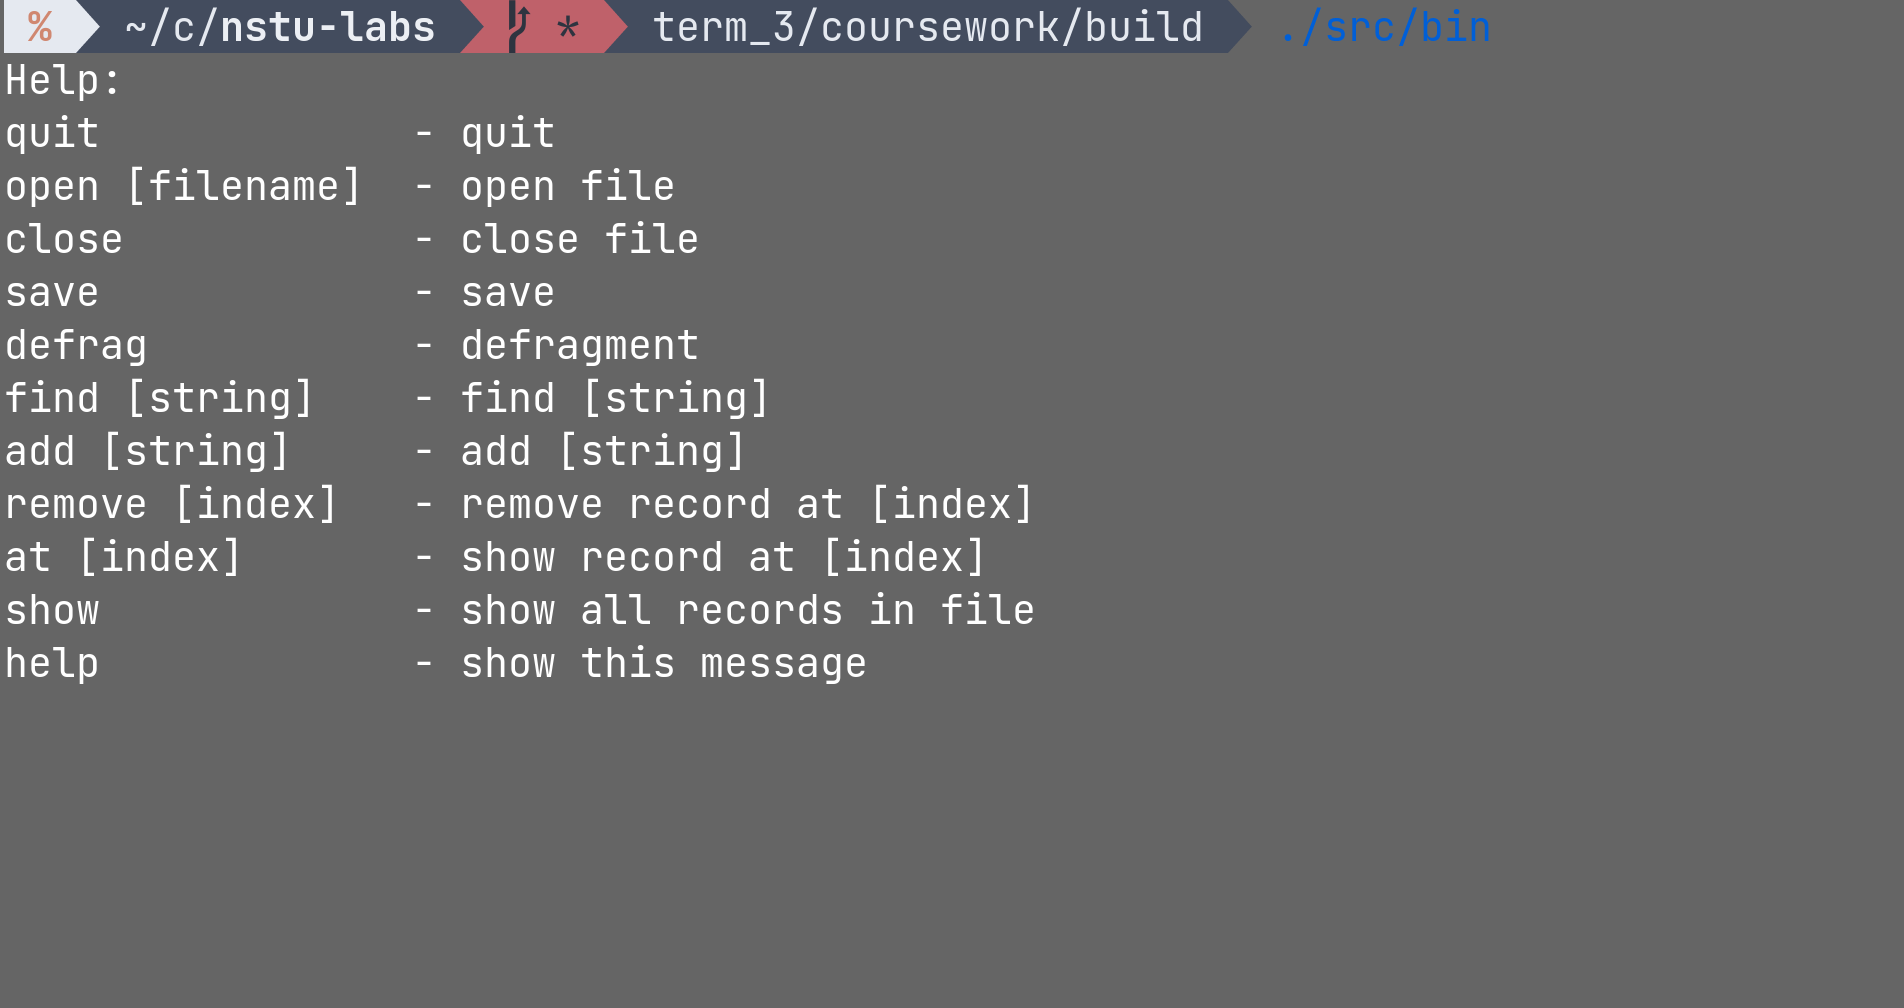
\includegraphics[width=\textwidth]{menu-main}
  \label{fig:menu-main}
  \caption{Меню программы.}
\end{figure}

\subsection{quit}
Сохраняет файл, если он был открыт и выходит.
\begin{figure}[H]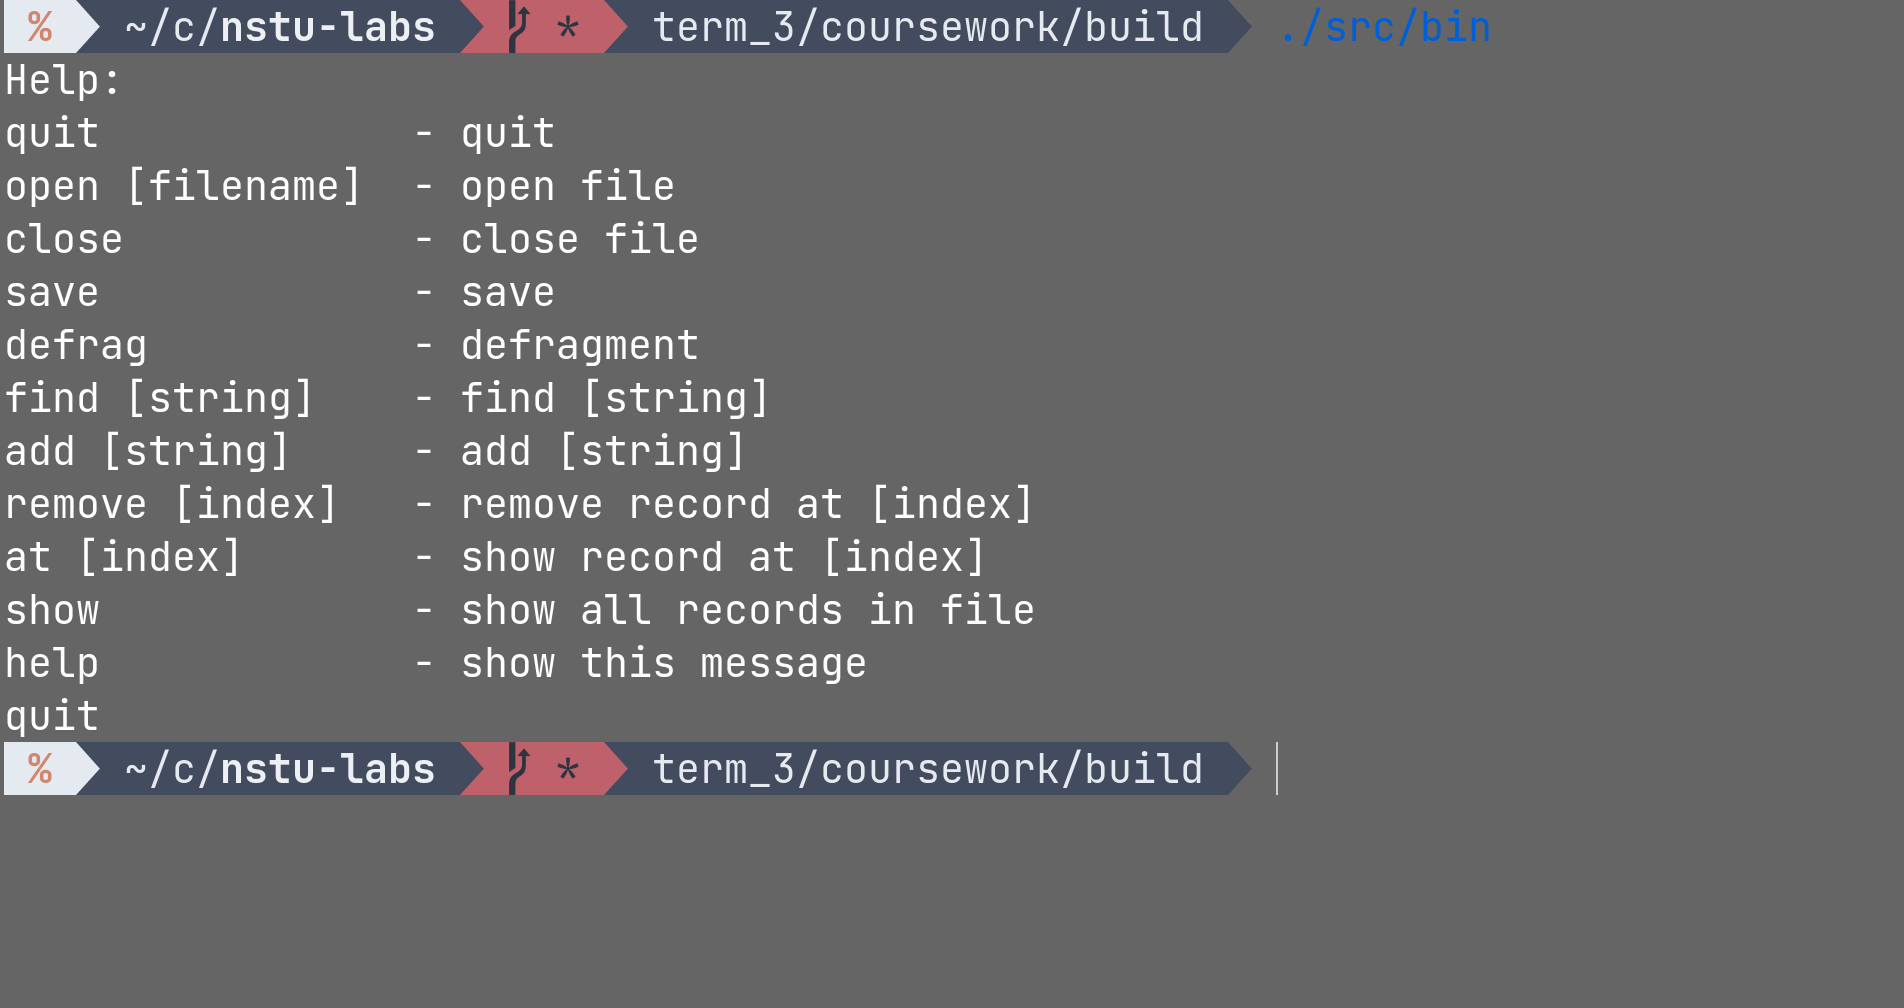
\includegraphics[width=\textwidth]{menu-quit}\label{fig:menu-quit}\caption{Выход из программы.}\end{figure}
\subsection{open [filename]}
Открывает файл, предварительно закрыв тот, что был открыт ранее (замена файла на другой).
\begin{figure}[H]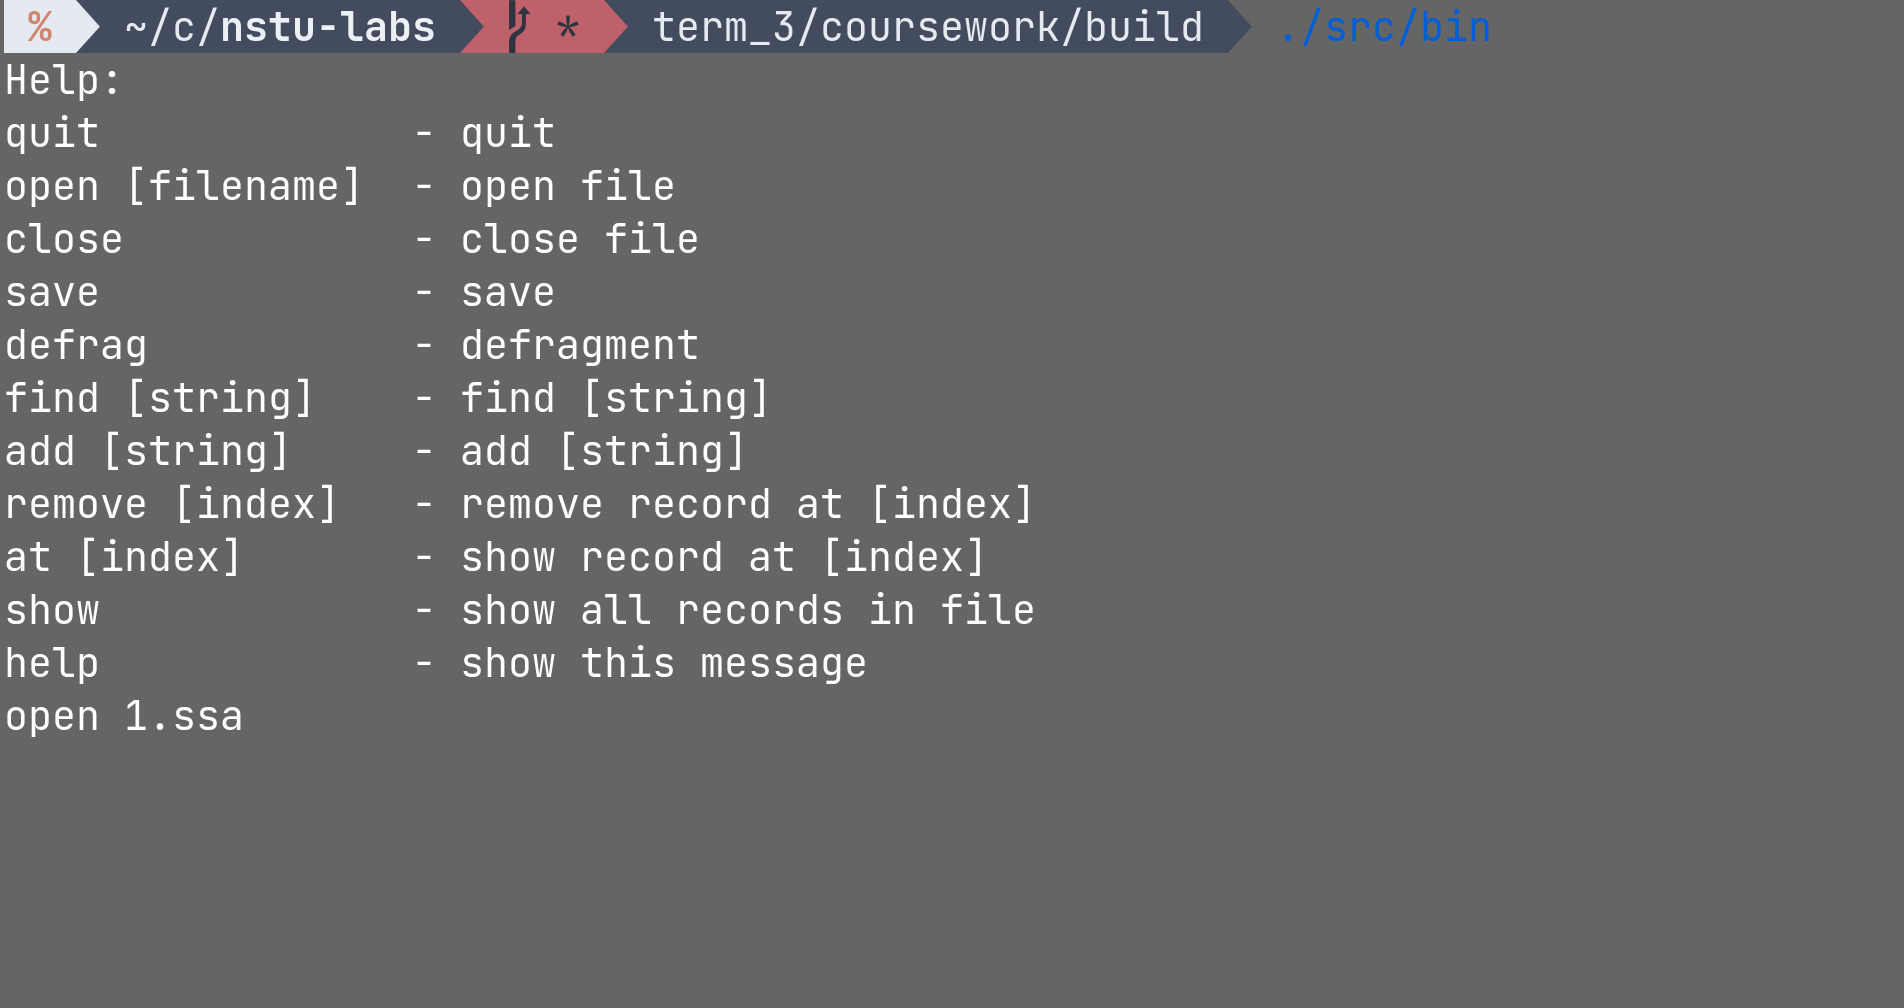
\includegraphics[width=\textwidth]{menu-open}\label{fig:menu-open}\caption{Открытие файла}\end{figure}
\subsection{close}
Закрывает файл, если он был открыт.
\begin{figure}[H]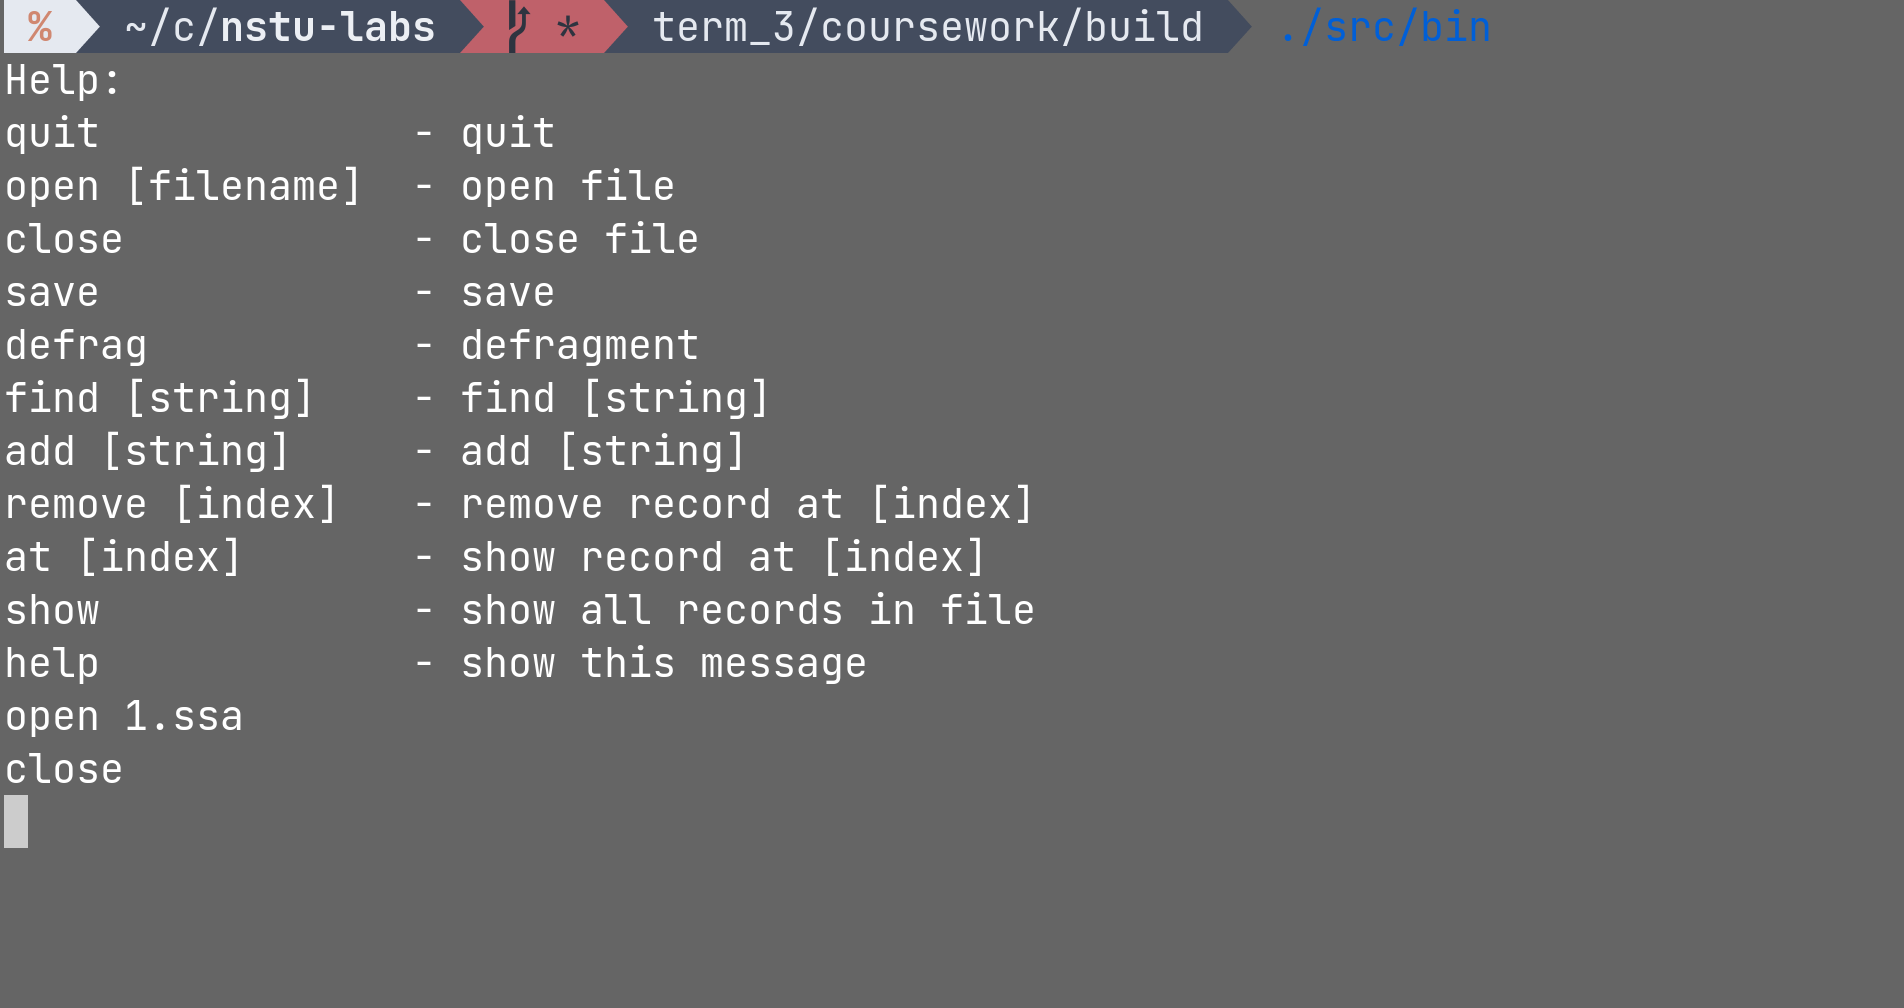
\includegraphics[width=\textwidth]{menu-close}\label{fig:menu-close}\caption{Закрытие файла.}\end{figure}
\subsection{save}
Сохраняет файл, если он был открыт.
\begin{figure}[H]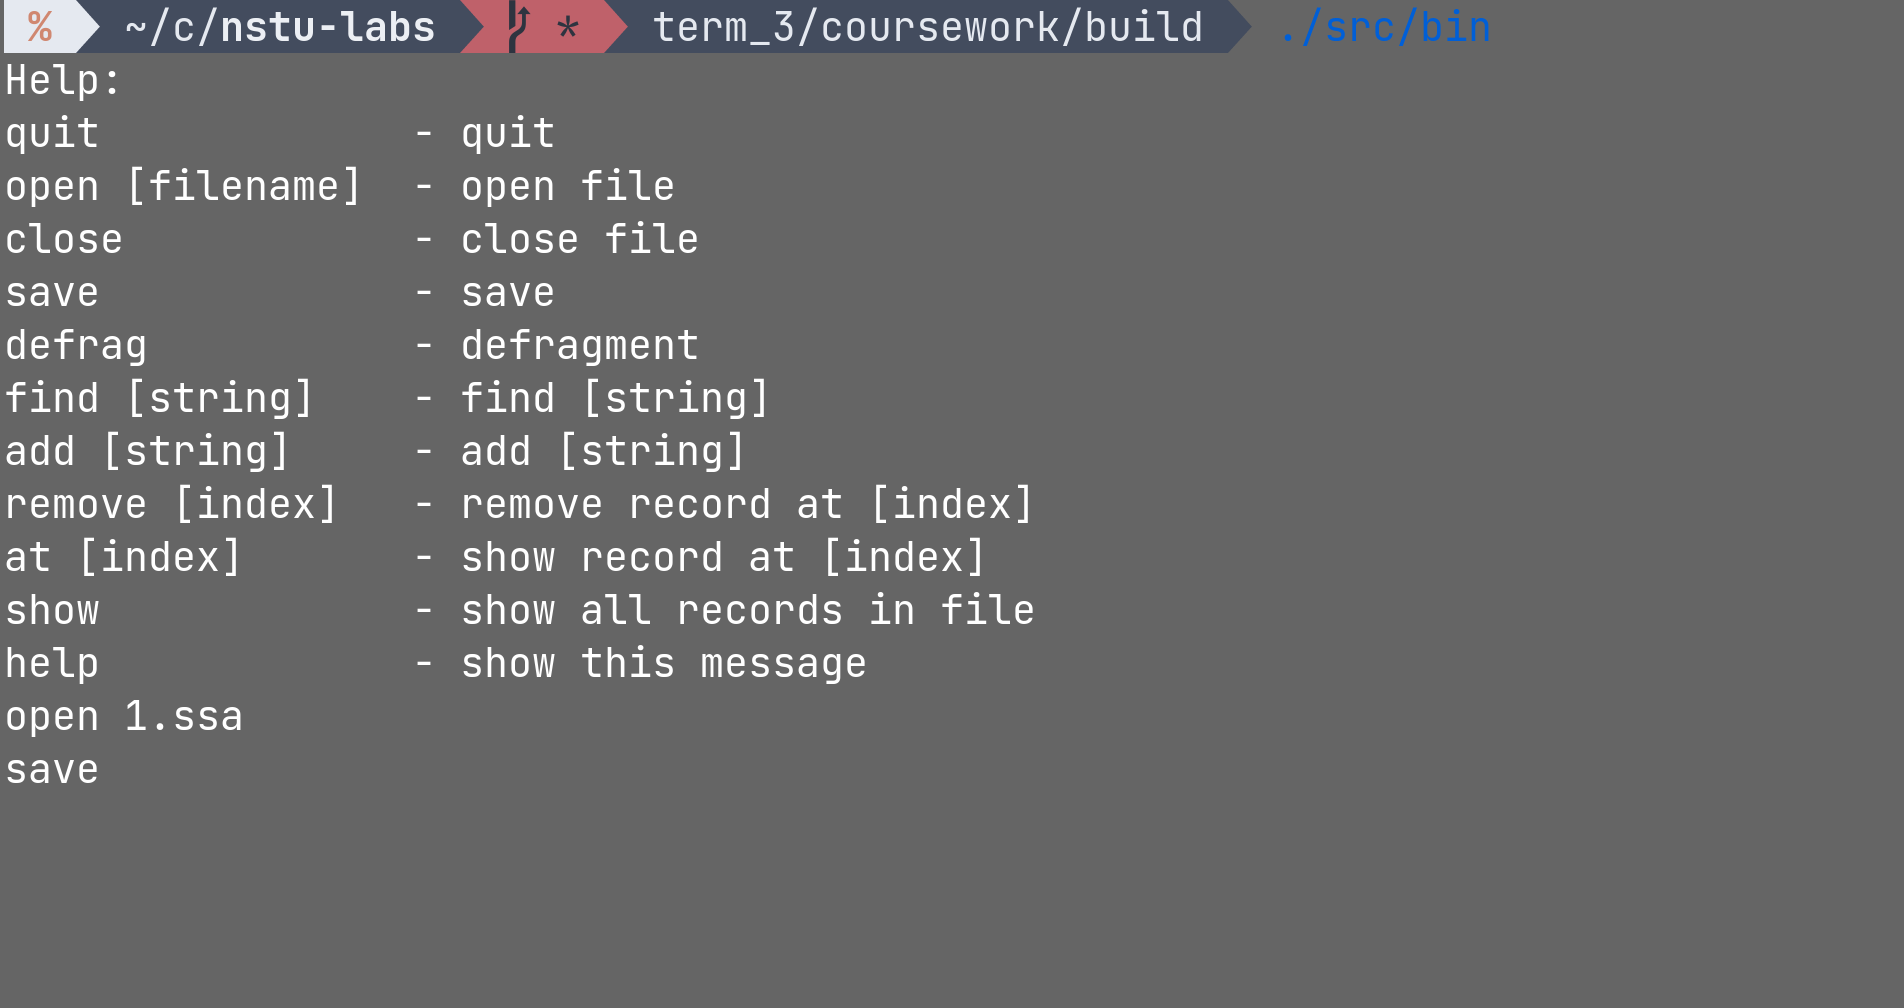
\includegraphics[width=\textwidth]{menu-save}\label{fig:menu-save}\caption{Сохранение файла.}\end{figure}
\subsection{defrag}
Производит дефрагментацию файла (\ref{sec:defrag}).
\begin{figure}[H]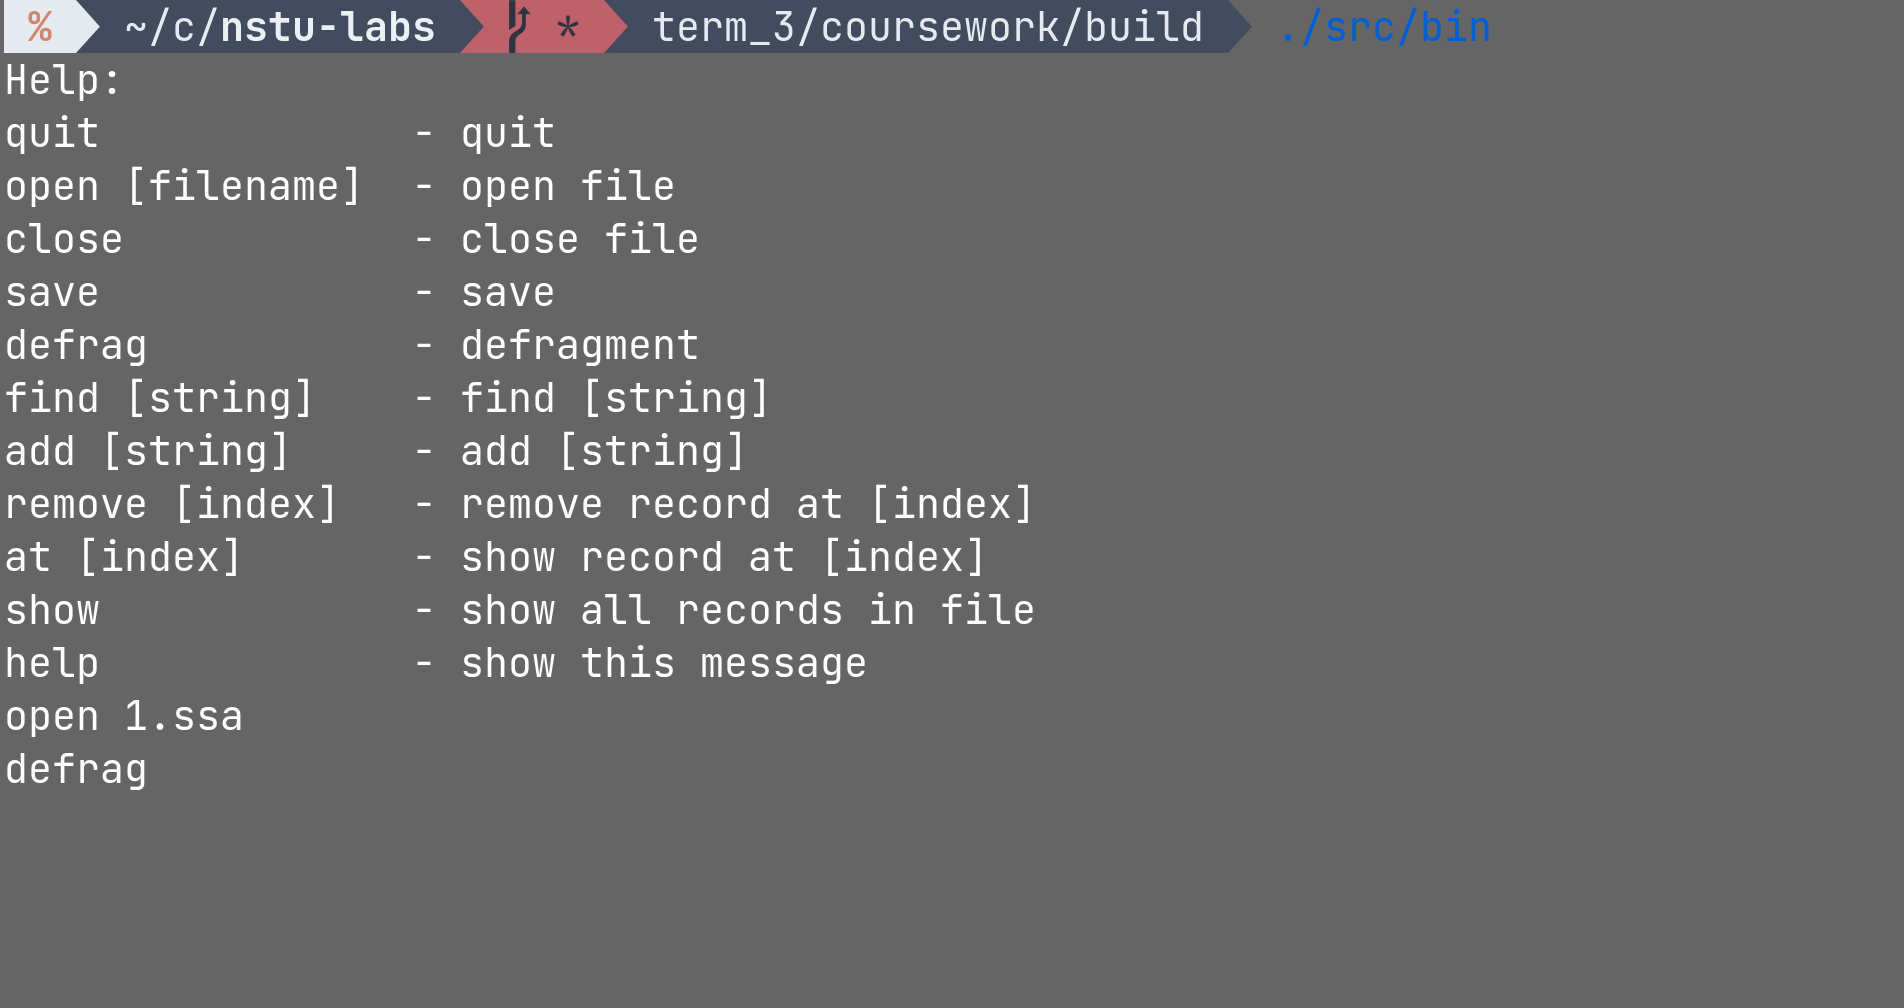
\includegraphics[width=\textwidth]{menu-defrag}\label{fig:menu-defrag}\caption{Дефрагментация файла.}\end{figure}
\subsection{show}
Выводит массив строк.
\begin{figure}[H]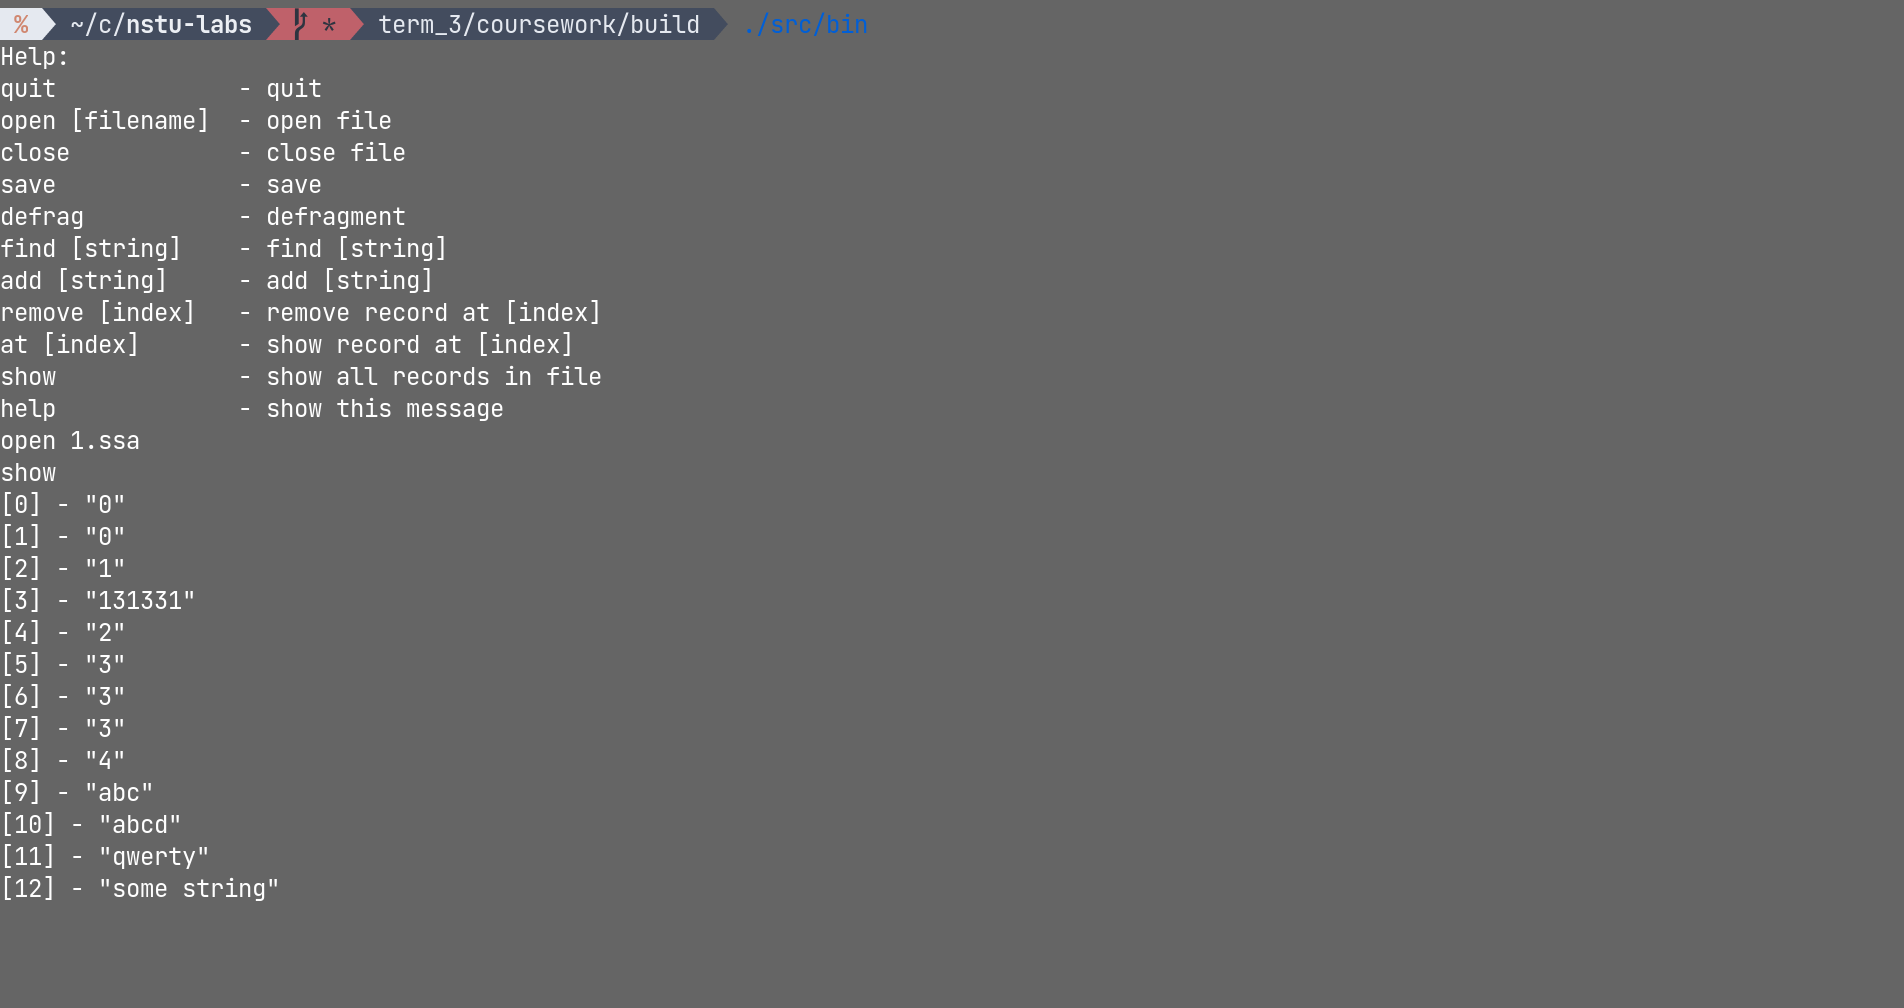
\includegraphics[width=\textwidth]{menu-show}\label{fig:menu-show}\caption{Дефрагментация файла.}\end{figure}
\subsection{find [string]}
Ищет строку в структуре данных, в случае, если строка не найдена выводит $-1$.
\begin{figure}[H]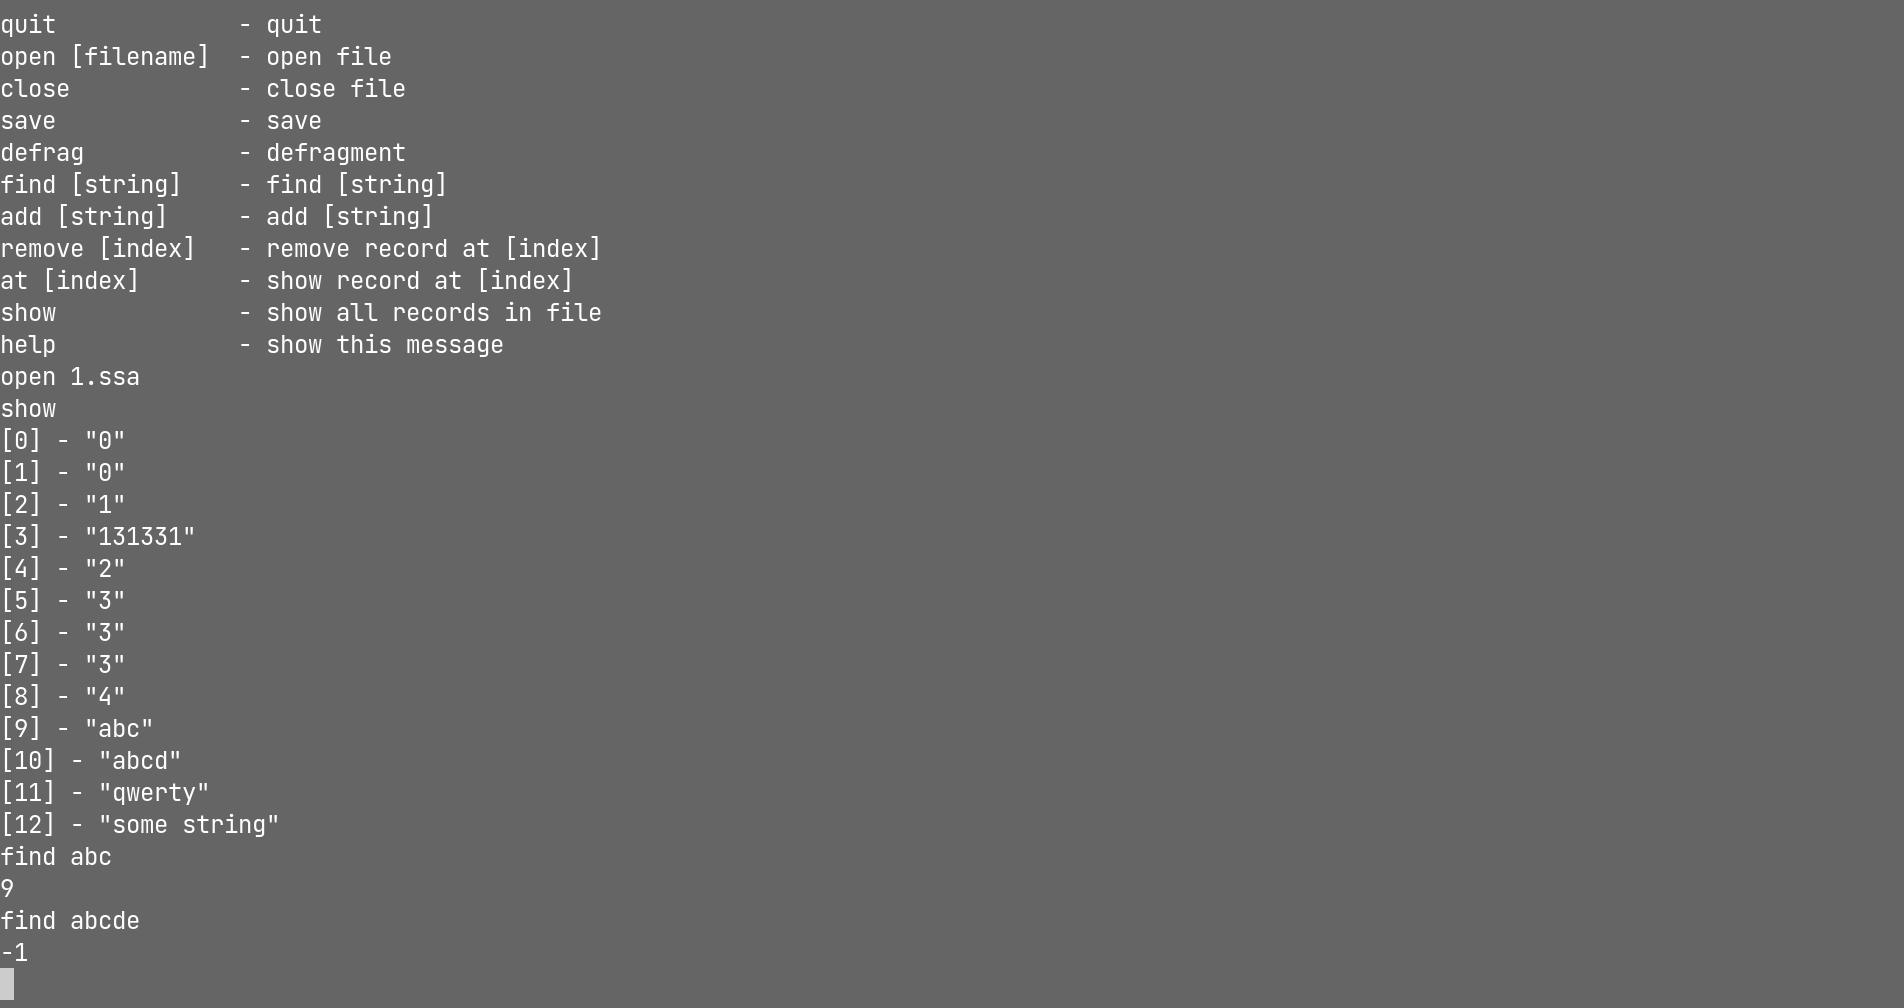
\includegraphics[width=\textwidth]{menu-find}\label{fig:menu-find}\caption{Дефрагментация файла.}\end{figure}
\subsection{add [string]}
Добавляет строку в структуру данных.
\begin{figure}[H]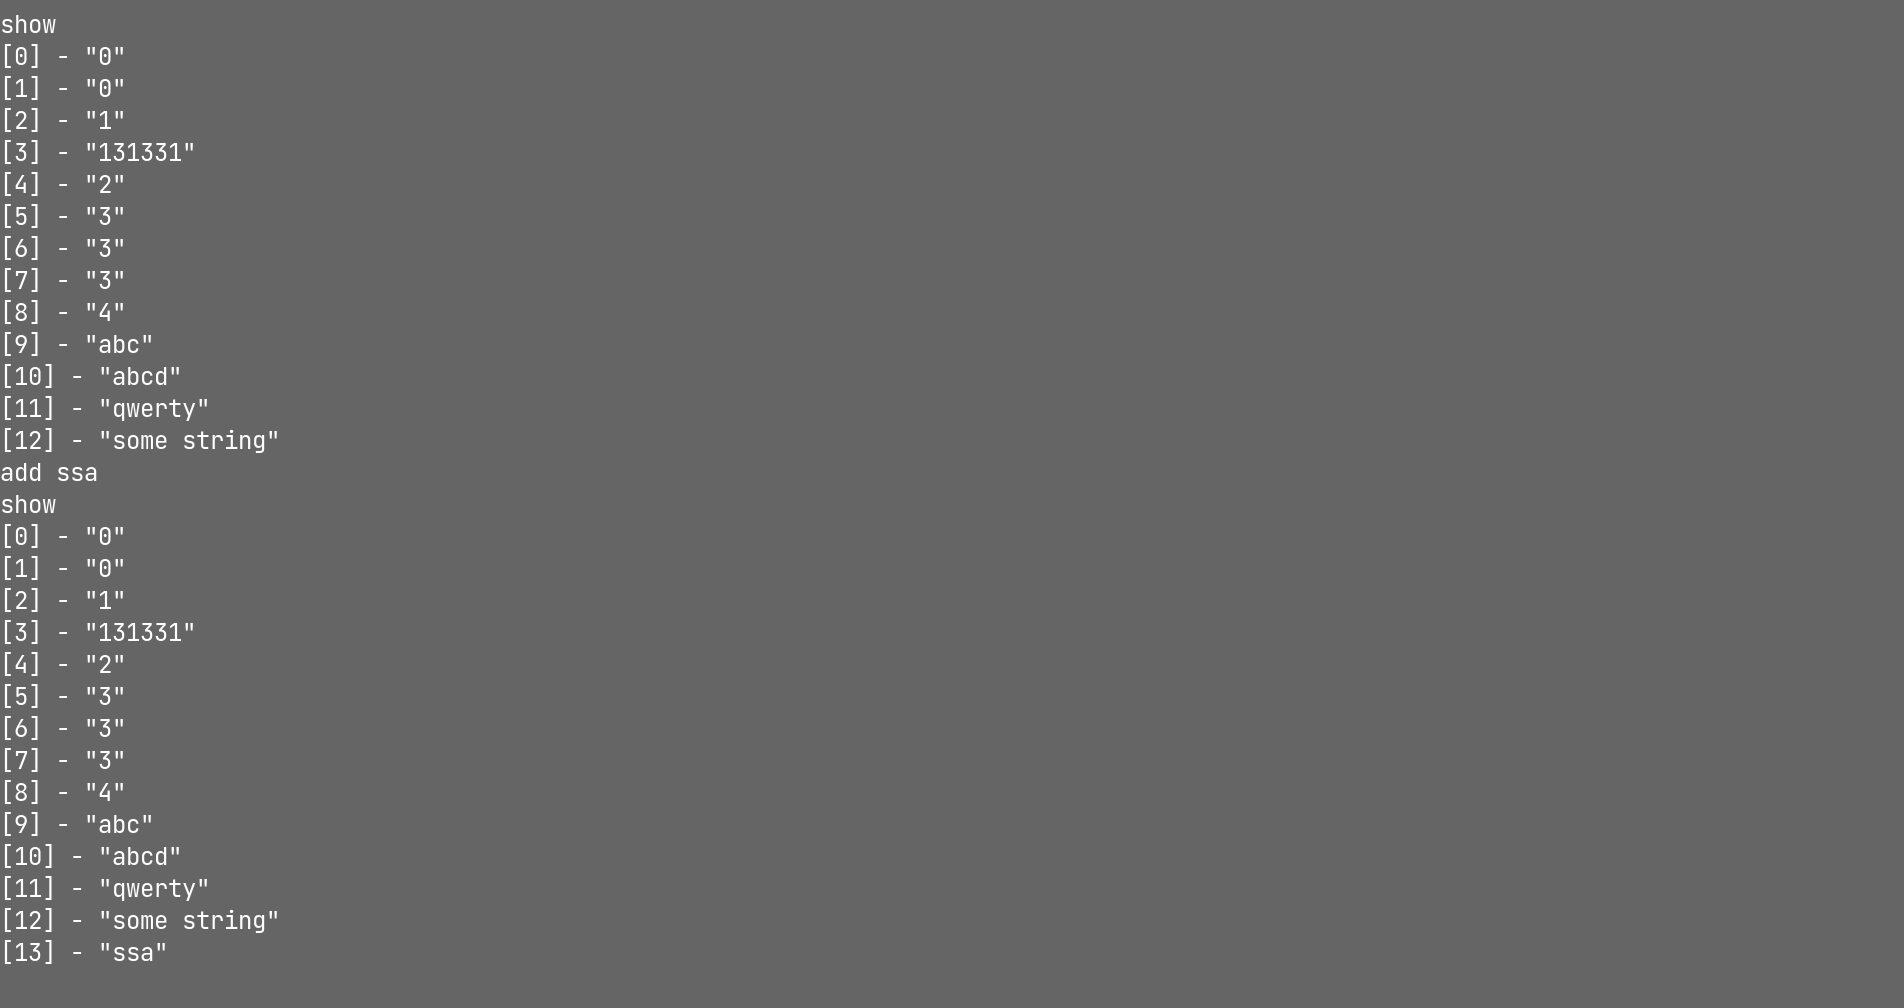
\includegraphics[width=\textwidth]{menu-add}\label{fig:menu-add}\caption{Добавление записи.}\end{figure}
\subsection{remove [index]}
Удаляет запись из структуры данных.
\begin{figure}[H]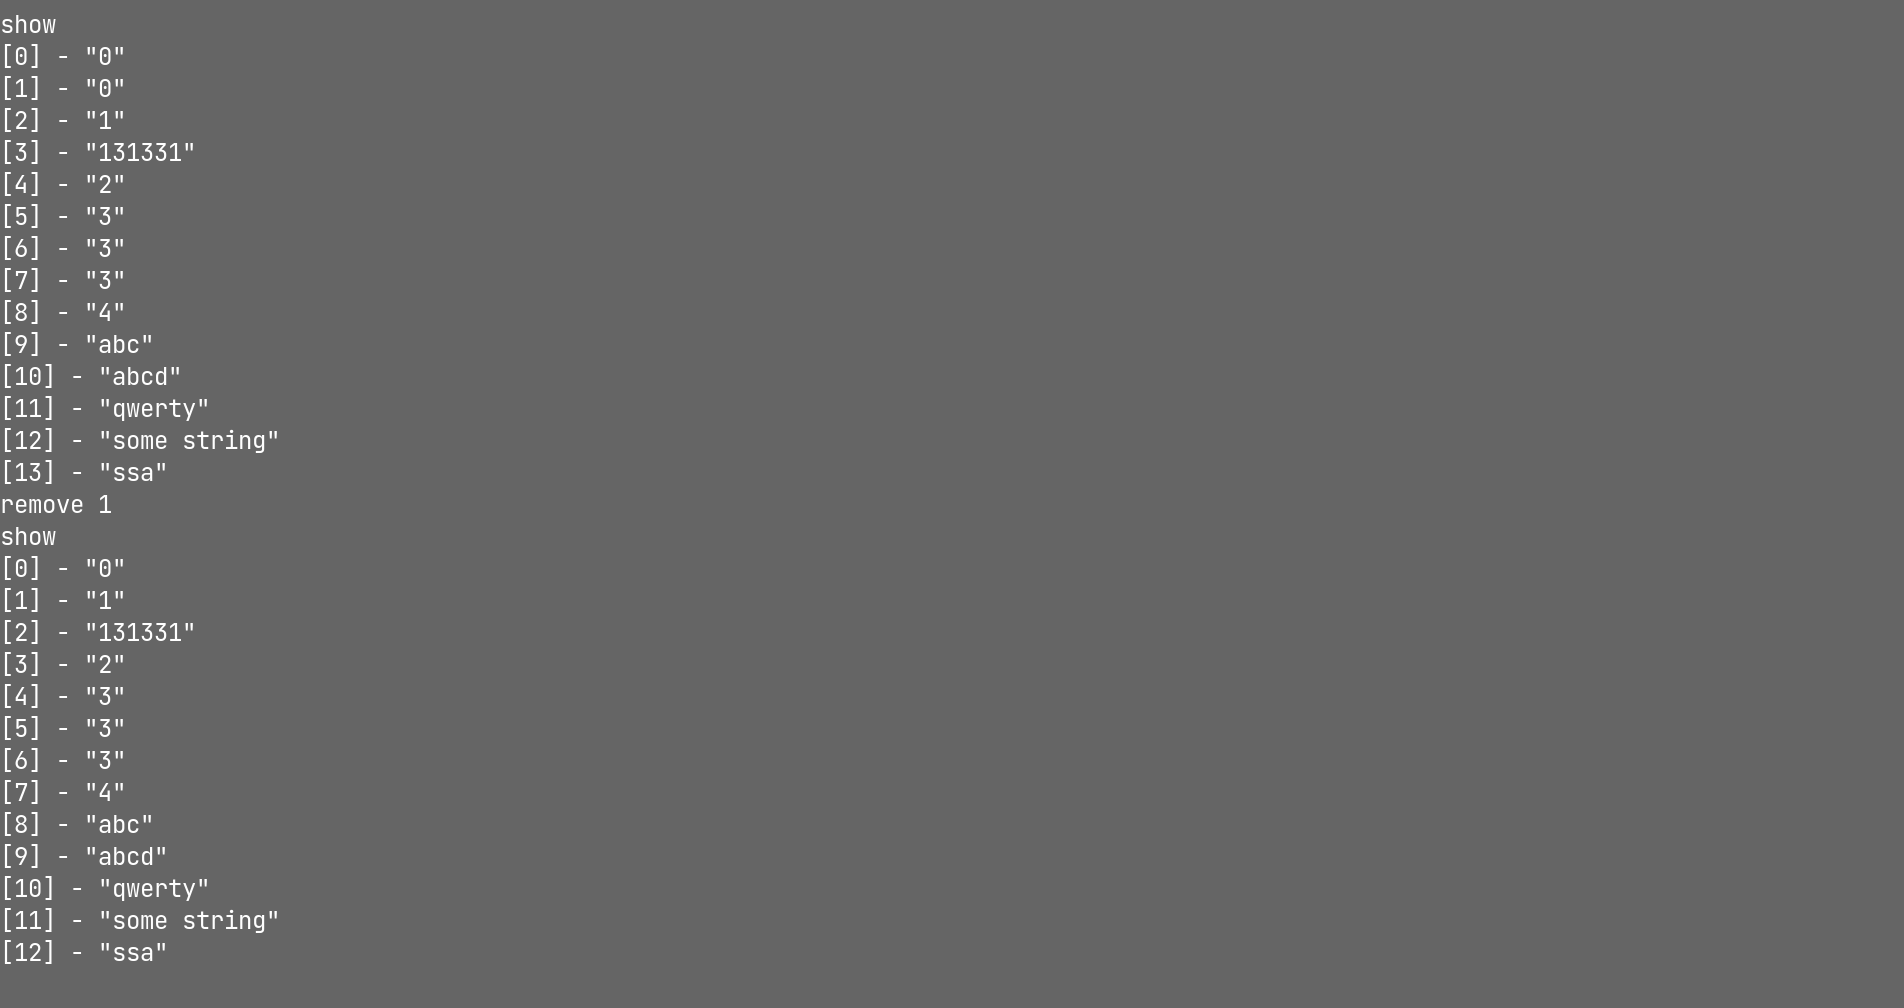
\includegraphics[width=\textwidth]{menu-remove}\label{fig:menu-remove}\caption{Удаление записи.}\end{figure}
\subsection{at [index]}
Получение значения по индексу.
\begin{figure}[H]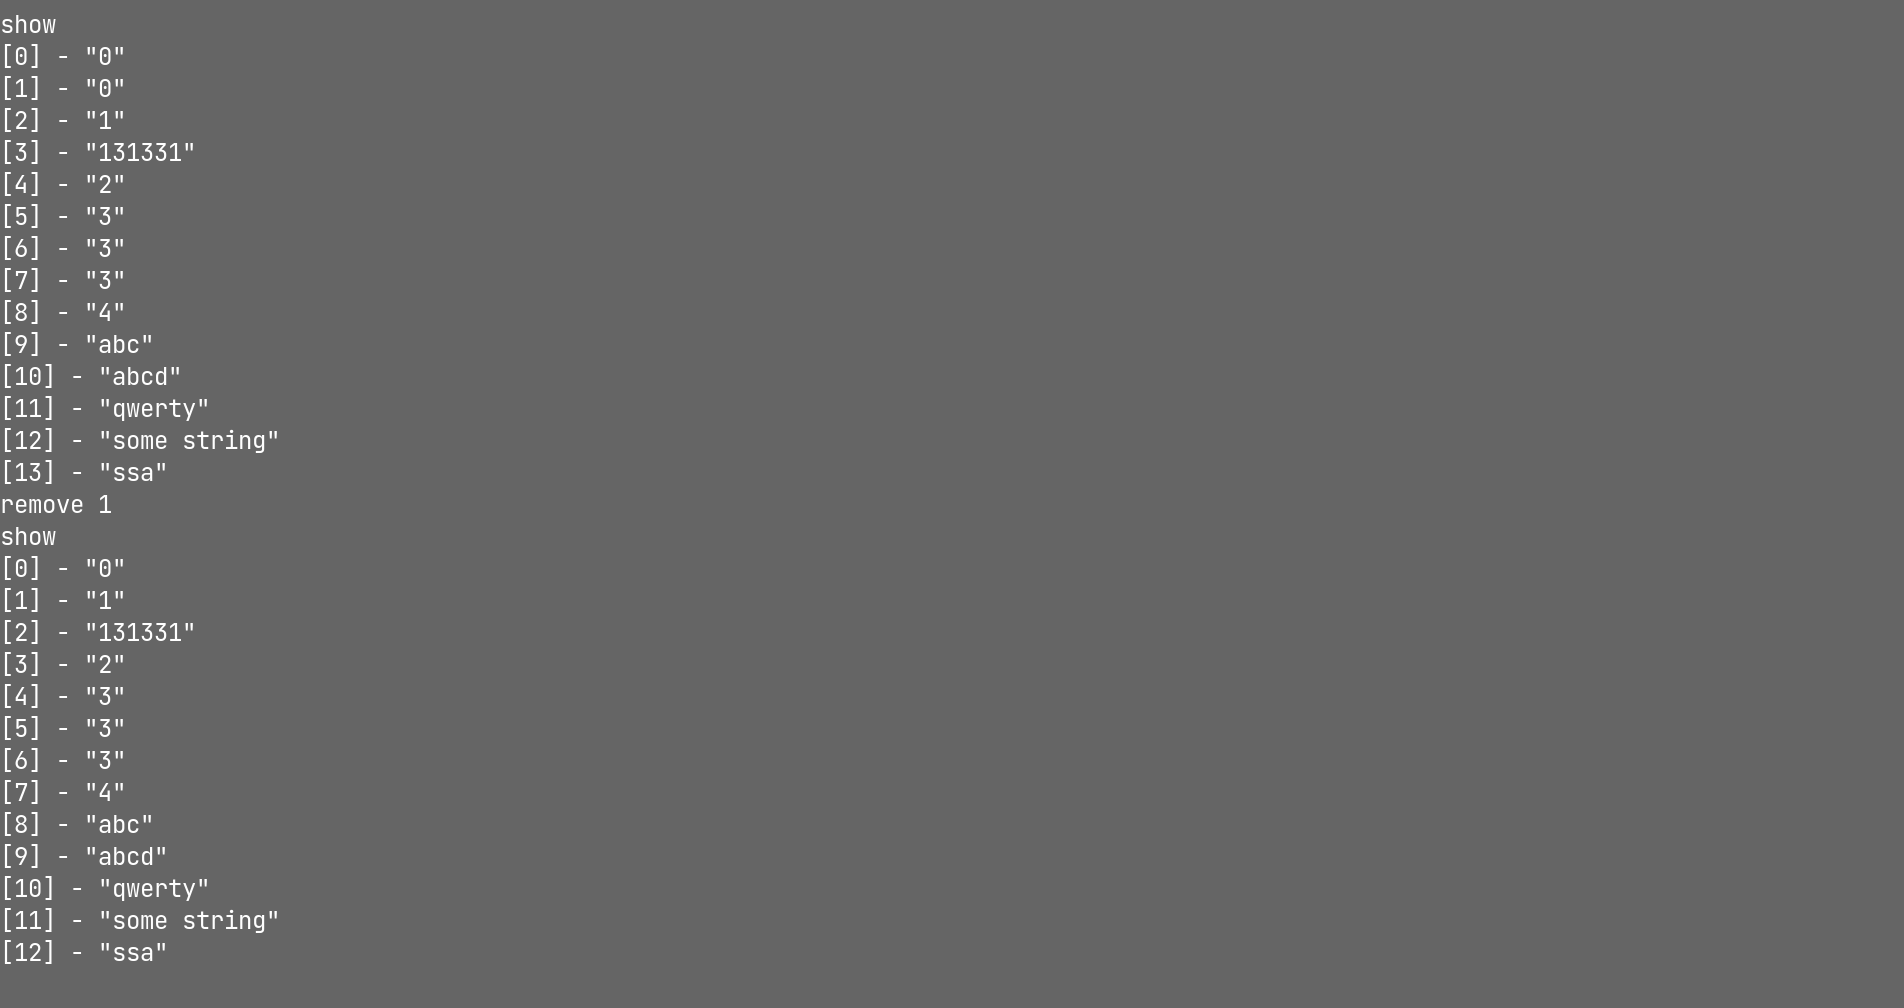
\includegraphics[width=\textwidth]{menu-remove}\label{fig:menu-remove}\caption{Получение записи по индексу}\end{figure}
\subsection{help}
Выводит список комманд и их краткое описание.
\begin{figure}[H]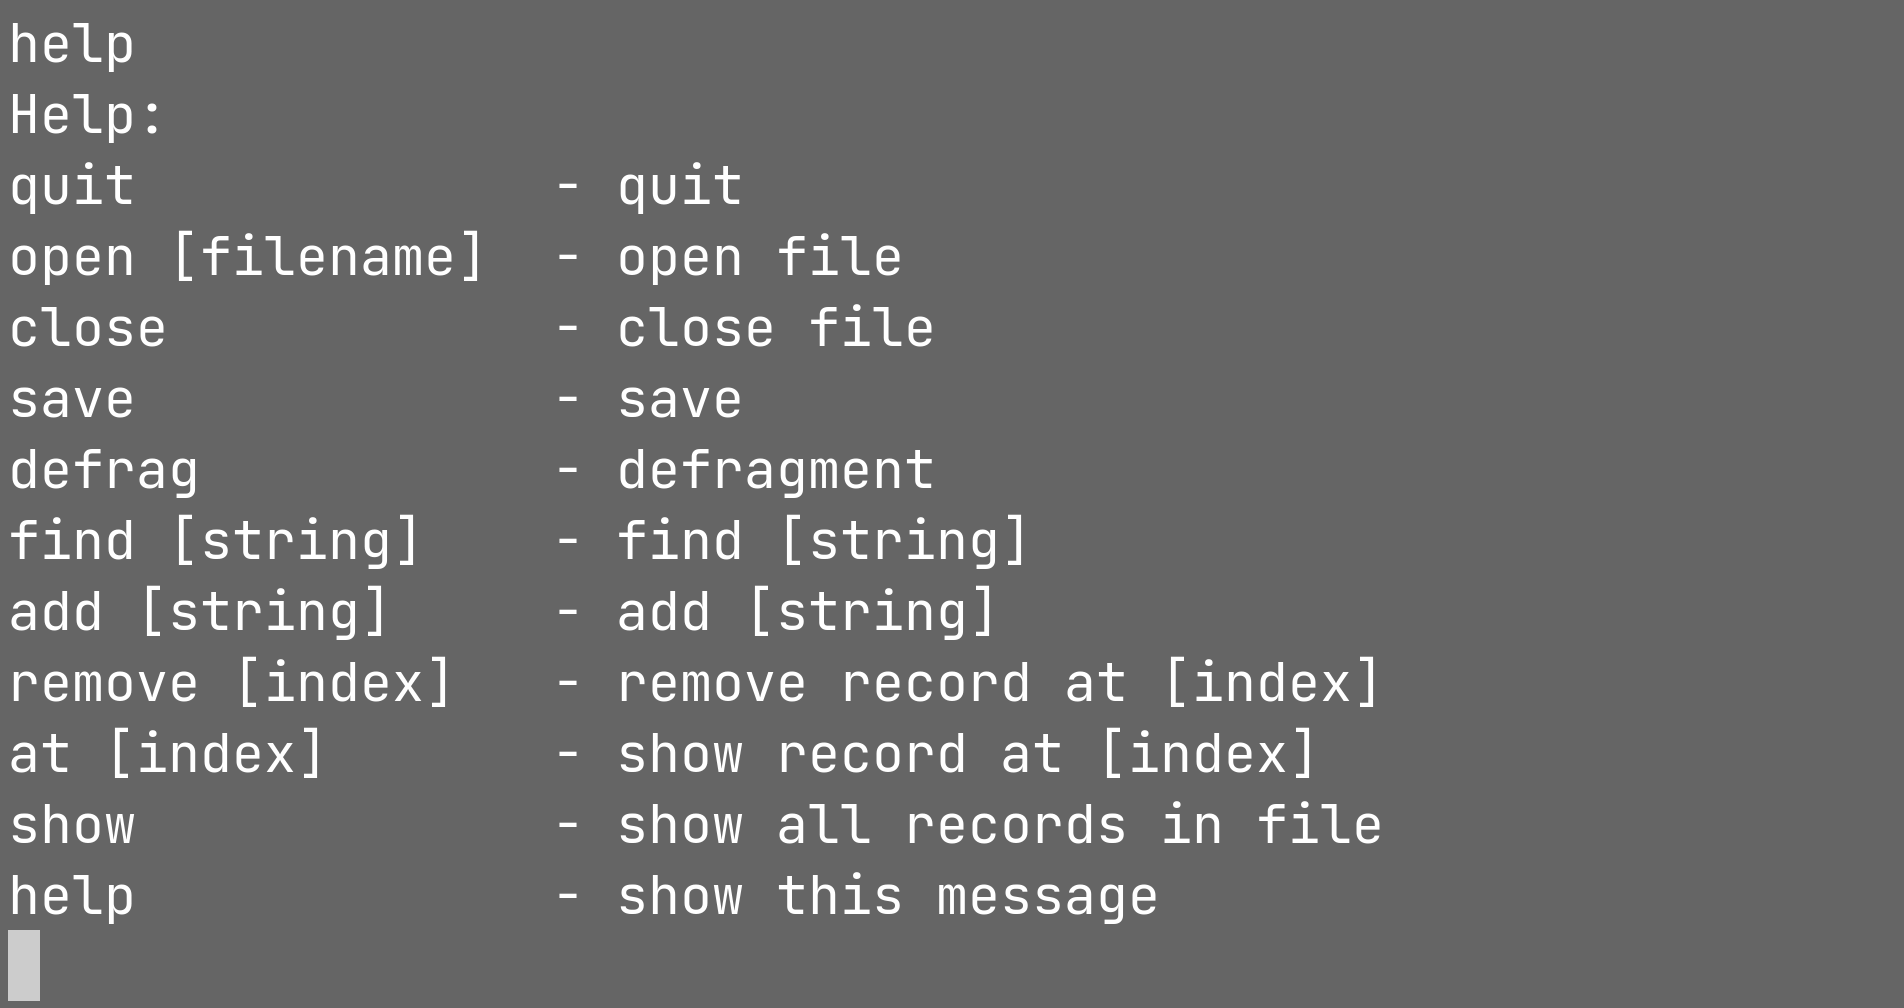
\includegraphics[width=\textwidth]{menu-help}\label{fig:menu-help}\caption{Список команд.}\end{figure}

\section{Скорость работы структуры данных}


Зависимость времени заполнения структуры одиннаковыми строками от их количества $n$ \\
\begin{tikzpicture}
  \begin{axis}[
    y label style={at={(axis description cs:-0.05,.5)}},
    xlabel={$n$},
    ylabel={$t$, мс},
    xmin=0, xmax=100000,
    ymin=0, ymax=5500,
    ymajorgrids=true,
    grid style=dashed,
    width=0.8\textwidth,
]

\addplot[color=blue,mark=square]coordinates{(10000, 505.777)
(20000, 1074.08)
(30000, 1453.15)
(40000, 2275.81)
(50000, 2621.96)
(60000, 3025.18)
(70000, 4361.79)
(80000, 4775.68)
(90000, 5342.96)
};
% \addlegendentry{Реальное время};
% \addplot[color=red,samples=100,domain=0:5000]{x*ln(x)/ln(2)};
% \addlegendentry{\(f(n) = n\log(n)\)};
% \addplot[color=green,samples=100,domain=0:5000]{x};
% \addlegendentry{\(f(n) = n\)};
\end{axis}
\end{tikzpicture}


Зависимость времени заполнения структуры различными строками от их количества $n$ (строки следуют друг за другом в лексикографическом порядке) \\
\begin{tikzpicture}
  \begin{axis}[
    y label style={at={(axis description cs:-0.05,.5)}},
    xlabel={$n$},
    ylabel={$t$, мс},
    xmin=0, xmax=10000,
    ymin=0, ymax=8900,
    ymajorgrids=true,
    grid style=dashed,
    width=0.8\textwidth,
]

\addplot[color=blue,mark=square]coordinates{(1000, 104.248)
(2000, 1718.04)
(3000, 3274.17)
(4000, 4656.45)
(5000, 5891.65)
(6000, 7121.23)
(7000, 7965.47)
(8000, 8191.04)
(9000, 8834.56)
};
% \addlegendentry{Реальное время};
% \addplot[color=red,samples=100,domain=0:10000]{x*ln(x)/ln(2)};
% \addlegendentry{\(f(n) = n\log(n)\)};
% \addplot[color=green,samples=100,domain=0:10000]{x};
% \addlegendentry{\(f(n) = n\)};
\end{axis}
\end{tikzpicture}

Зависимость времени заполнения структуры различными строками от их количества $n$ (строки не следуют в лексикографическом порядке) \\
\begin{tikzpicture}
  \begin{axis}[
    y label style={at={(axis description cs:-0.05,.5)}},
    xlabel={$n$},
    ylabel={$t$, мс},
    xmin=0, xmax=5000,
    ymin=0, ymax=9500,
    ymajorgrids=true,
    grid style=dashed,
    width=0.8\textwidth,
]

\addplot[color=blue,mark=square]coordinates{(500, 140.056)
(1000, 453.292)
(1500, 1108.19)
(2000, 2076.88)
(2500, 3204.58)
(3000, 4239.93)
(3500, 5755.9)
(4000, 7083.13)
(4500, 9329.02)
};
% \addlegendentry{Реальное время};
% \addplot[color=red,samples=100,domain=0:5000]{x*ln(x)/ln(2)};
% \addlegendentry{\(f(n) = n\log(n)\)};
% \addplot[color=green,samples=100,domain=0:5000]{x};
% \addlegendentry{\(f(n) = n\)};
\end{axis}
\end{tikzpicture}

Проанализировав графики можно сделать выводы, что на одиннаковых данных и данных, идущих в лексикографическом порядке, структура данных ведет себя как прямая. Хоть и ассимптотически зависимость должна быть логарифмическая, т.к. в таком случае вставка занимает $O(1)$, но из-за расширений массива оно сводится к линейной в полученных частных случаях. В случае случайных данных следует еще и за $O(n)$ вставлять элементы в массив, что придает зависимости экспоненциальный вид, но довольно близкий к прямой линии, т.к. расширения массива происходят все реже.


  \newpage
  \section*{Заключение}\label{sec:end}\addcontentsline{toc}{section}{\nameref{sec:end}}
  В результате выполнения работы была спроектирована и реализована структура данных, представляющая собой массив строк в лексикографическом порядке, хранящимся, используя парадигму объектно-ориентированного программирования. \linebreak
  \indent В частности, для структуры данных был разработан пользовательский интерфейс, с помощью которого она была протестирована.
  Задание предполагает наследование от класса \textit{std::fstream}, что позволяет расширять функционал класса и что несомненно является преимуществом объектно-ориентированной парадигмы программирования.

  \section*{Приложения}\label{sec:application}\addcontentsline{toc}{section}{\nameref{sec:application}}
  \subsection*{Листинг программы}\label{sec:application1}\addcontentsline{toc}{section}{\nameref{sec:application1}}

  \textit{main.cpp}
  \inputminted{cpp}{../src/main.cpp}
  \textit{sorted\_string\_array.hpp}
  \inputminted{cpp}{../src/sorted_string_array.hpp}
  \textit{sorted\_string\_array.cpp}
  \inputminted{cpp}{../src/sorted_string_array.cpp}
  \textit{commands.hpp}
  \inputminted{cpp}{../src/commands.hpp}
  \textit{commands.cpp}
  \inputminted{cpp}{../src/commands.cpp}


\end{document}
